%%%%%%%%%%%%%%%%%%%%%%%%%%%%%%%%%%%%%%%%%
% Masters/Doctoral Thesis 
% LaTeX Template
% Version 2.5 (27/8/17)
%
% This template was downloaded from:
% http://www.LaTeXTemplates.com
%
% Version 2.x major modifications by:
% Vel (vel@latextemplates.com)
%
% This template is based on a template by:
% Steve Gunn (http://users.ecs.soton.ac.uk/srg/softwaretools/document/templates/)
% Sunil Patel (http://www.sunilpatel.co.uk/thesis-template/)
%
% Template license:
% CC BY-NC-SA 3.0 (http://creativecommons.org/licenses/by-nc-sa/3.0/)
%
%%%%%%%%%%%%%%%%%%%%%%%%%%%%%%%%%%%%%%%%%

%----------------------------------------------------------------------------------------
%	PACKAGES AND OTHER DOCUMENT CONFIGURATIONS
%----------------------------------------------------------------------------------------

\documentclass[
12pt, % The default document font size, options: 10pt, 11pt, 12pt
oneside, % Two side (alternating margins) for binding by default, uncomment to switch to one side
english, % ngerman for German
singlespacing, % Single line spacing, alternatives: onehalfspacing or doublespacing
%draft, % Uncomment to enable draft mode (no pictures, no links, overfull hboxes indicated)
%nolistspacing, % If the document is onehalfspacing or doublespacing, uncomment this to set spacing in lists to single
%liststotoc, % Uncomment to add the list of figures/tables/etc to the table of contents
%toctotoc, % Uncomment to add the main table of contents to the table of contents
%parskip, % Uncomment to add space between paragraphs
%nohyperref, % Uncomment to not load the hyperref package
headsepline, % Uncomment to get a line under the header
%chapterinoneline, % Uncomment to place the chapter title next to the number on one line
%consistentlayout, % Uncomment to change the layout of the declaration, abstract and acknowledgements pages to match the default layout
]{MastersDoctoralThesis} % The class file specifying the document structure

\usepackage[utf8]{inputenc} % Required for inputting international characters
\usepackage[T1]{fontenc} % Output font encoding for international characters

\usepackage{mathpazo} % Use the Palatino font by default

\usepackage[backend=bibtex,style=authoryear,natbib=true, maxbibnames=99]{biblatex} % Use the bibtex backend with the authoryear citation style (which resembles APA)

%---below is to make the et al italics....
\xpatchbibmacro{name:andothers}{%
  \bibstring{andothers}%
}{%
  \bibstring[\emph]{andothers}%
}{}{}

\addbibresource{example.bib} % The filename of the bibliography

\usepackage[autostyle=true]{csquotes} % Required to generate language-dependent quotes in the bibliography

%---Force image to appear in its section
\usepackage[section]{placeins}

%---To indicate that certain texts are comments
\usepackage{comment}

%---To change default bullet points
\usepackage{amssymb}

% Required packages to your document preamble for table
\usepackage{booktabs}

\usepackage{tabu}

%---This is for APA style for referencing figures
\captionsetup[figure]{labelsep=period,labelfont=it,justification=justified,singlelinecheck=false,font=singlespacing}
 
 %---This is for APA style for referencing tables 
 \DeclareCaptionLabelSeparator*{spaced}{\\[2ex]}
  \captionsetup[table]{textfont=it,format=plain,justification=justified,singlelinecheck=false,labelsep=spaced,skip=10pt}

%----------------------------------------------------------------------------------------
%	MARGIN SETTINGS
%----------------------------------------------------------------------------------------

\geometry{
	paper=a4paper, % Change to letterpaper for US letter
	inner=1.5cm, % Inner margin
	outer=2.5cm, % Outer margin
	bindingoffset=2cm, % Binding offset
	top=1.5cm, % Top margin
	bottom=1.5cm, % Bottom margin
	%showframe, % Uncomment to show how the type block is set on the page
}

%----------------------------------------------------------------------------------------
%	THESIS INFORMATION
%----------------------------------------------------------------------------------------

\thesistitle{Using Technology To Support Mothers Of Premature Infants} % Your thesis title, this is used in the title and abstract, print it elsewhere with \ttitle
\supervisor{Dr. Melissa \textsc{Densmore}\\ Dr. Yaseen \textsc{Joolay}} % Your supervisor's name, this is used in the title page, print it elsewhere with \supname
\examiner{} % Your examiner's name, this is not currently used anywhere in the template, print it elsewhere with \examname
\degree{Doctor of Philosophy} % Your degree name, this is used in the title page and abstract, print it elsewhere with \degreename
\author{Christine Wanjiru \textsc{Mburu}} % Your name, this is used in the title page and abstract, print it elsewhere with \authorname
\addresses{} % Your address, this is not currently used anywhere in the template, print it elsewhere with \addressname

\subject{Computer Science} % Your subject area, this is not currently used anywhere in the template, print it elsewhere with \subjectname
\keywords{} % Keywords for your thesis, this is not currently used anywhere in the template, print it elsewhere with \keywordnames
\university{\href{https://www.uct.ac.za/}{University of Cape Town}} % Your university's name and URL, this is used in the title page and abstract, print it elsewhere with \univname
\department{\href{https://www.cs.uct.ac.za/}{Department of Computer Science}} % Your department's name and URL, this is used in the title page and abstract, print it elsewhere with \deptname
%\group{\href{http://researchgroup.university.com}{Research Group Name}} % Your research group's name and URL, this is used in the title page, print it elsewhere with \groupname
\faculty{\href{http://www.science.uct.ac.za/}{Faculty of Science}} % Your faculty's name and URL, this is used in the title page and abstract, print it elsewhere with \facname

\AtBeginDocument{
\hypersetup{pdftitle=\ttitle} % Set the PDF's title to your title
\hypersetup{pdfauthor=\authorname} % Set the PDF's author to your name
\hypersetup{pdfkeywords=\keywordnames} % Set the PDF's keywords to your keywords
}
\hyphenation{ac-ti-vi-ties Ua-ri-ai-ke ova-Him-ba ova-He-re-ro ova-Tjim-ba}

\usepackage[acronym, toc]{glossaries}

\makeglossaries

% Here is to generate a glossary (Words used in the Thesis with their explanations)
%
\newglossaryentry{IKholder}
{
    name=IK holder,
    description={Seniors from 30 years old or lower who have mastered the indigenous knowledge of their communities}
}

\newglossaryentry{kraal}
{
    name=kraal,
    description={Kraal is an Afrikaans and Dutch word for a fenced area for keeping livestock for proper management}
}

\newglossaryentry{holyFire}
{
    name=holy-fire,
    description={Known as \emph{okuruo} in Otjiherero is a sacred place where the Otjiherero speaking elders pray to God through their ancestors}
}



% End of Glossary !

% Begin acronym declaration !

\newacronym{uct}{UCT}{University of Cape Town}

\newacronym{gsh}{GSH}{Groote Schuur Hospital}

\newacronym{nicu}{NICU}{Neonatal Intensive Care Unit}

\newacronym{hci}{HCI}{Human-Computer Interaction}

\newacronym{hci4d}{HCI4D}{Human-Computer Interaction for Development}

\newacronym{chi}{CHI}{Computer Human Interaction}

\newacronym{pd}{PD}{Participatory Design}

\newacronym{ict}{ICT}{Information Communication Technology}

\newacronym{ict4d}{ICT4D}{Information Communication Technology for Development}

\newacronym{icu1}{ICU1}{Intensive Care Unit 1}

\newacronym{icu2}{ICU2}{Intensive Care Unit 2}

\newacronym{hc1}{HC1}{High Care 1}

\newacronym{hc2}{HC2}{High Care 2}

%-------------End of Acronyms !---------

\includecomment{comment}

\begin{document}

\frontmatter % Use roman page numbering style (i, ii, iii, iv...) for the pre-content pages

\pagestyle{plain} % Default to the plain heading style until the thesis style is called for the body content

%----------------------------------------------------------------------------------------
%	TITLE PAGE
%----------------------------------------------------------------------------------------

\begin{titlepage}
\begin{center}


\includegraphics[width=0.30\textwidth]{Figures/uct-logo.png} % University/department logo - uncomment to place it

\vspace*{.06\textheight}
{\scshape\LARGE \univname\par}\vspace{1.0cm} % University name
\textsc{\Large Doctoral Thesis}\\[0.5cm] % Thesis type

\HRule \\[0.4cm] % Horizontal line
{\huge \bfseries \ttitle\par}\vspace{0.4cm} % Thesis title
\HRule \\[1.5cm] % Horizontal line
 
\begin{minipage}[t]{0.4\textwidth}
\begin{flushleft} \large
\emph{Author:}\\
\href{http://www.johnsmith.com}{\authorname} % Author name - remove the \href bracket to remove the link
\end{flushleft}
\end{minipage}
\begin{minipage}[t]{0.4\textwidth}
\begin{flushright} \large
\emph{Supervisor:} \\
\href{https://people.cs.uct.ac.za/~melissa}{\supname} % Supervisor name - remove the \href bracket to remove the link  
\end{flushright}
\end{minipage}\\[1cm]
 
\vfill

\large \textit{A thesis submitted in fulfillment of the requirements\\ for the degree of \degreename}\\[0.3cm] % University requirement text
\textit{in the}\\[0.4cm]
\deptname\\[0.4cm] % Research group name and department name
{\large \today}\\[2cm] % Date
\end{center}
\end{titlepage}

%----------------------------------------------------------------------------------------
%	DECLARATION PAGE
%----------------------------------------------------------------------------------------

\begin{declaration}
\addchaptertocentry{\authorshipname} % Add the declaration to the table of contents
\noindent I, \authorname, declare that this thesis titled, \enquote{\ttitle} and the work presented in it are my own. I confirm that:

\begin{itemize} 
\item This work was done wholly or mainly while in candidature for a research degree at this University.
\item Where any part of this thesis has previously been submitted for a degree or any other qualification at this University or any other institution, this has been clearly stated.
\item Where I have consulted the published work of others, this is always clearly attributed.
\item Where I have quoted from the work of others, the source is always given. With the exception of such quotations, this thesis is entirely my own work.
\item I have acknowledged all main sources of help.
\item Where the thesis is based on work done by myself jointly with others, I have made clear exactly what was done by others and what I have contributed myself.\\
\end{itemize}
 
\noindent Signed:\\
\rule[0.5em]{25em}{0.5pt} % This prints a line for the signature
 
\noindent Date:\\
\rule[0.5em]{25em}{0.5pt} % This prints a line to write the date
\end{declaration}

\cleardoublepage

%----------------------------------------------------------------------------------------
%	QUOTATION PAGE
%----------------------------------------------------------------------------------------

\vspace*{0.2\textheight}

\noindent\enquote{\itshape Thanks to my solid academic training, today I can write hundreds of words on virtually any topic without possessing a shred of information, which is how I got a good job in journalism.}\bigbreak

\hfill Dave Barry

%----------------------------------------------------------------------------------------
%	ABSTRACT PAGE
%----------------------------------------------------------------------------------------

\begin{abstract}
\addchaptertocentry{\abstractname} % Add the abstract to the table of contents
ADD ABSTRACT
\end{abstract}

%----------------------------------------------------------------------------------------
%	ACKNOWLEDGEMENTS
%----------------------------------------------------------------------------------------

\begin{acknowledgements}
\addchaptertocentry{\acknowledgementname} % Add the acknowledgements to the table of contents
The acknowledgments and the people to thank go here, don't forget to include your project advisor\ldots
\end{acknowledgements}

%----------------------------------------------------------------------------------------
%	LIST OF CONTENTS/FIGURES/TABLES PAGES
%----------------------------------------------------------------------------------------

\tableofcontents % Prints the main table of contents

\listoffigures % Prints the list of figures

\listoftables % Prints the list of tables

%----------------------------------------------------------------------------------------
%	ABBREVIATIONS
%----------------------------------------------------------------------------------------

\printglossary
\printglossary[type=\acronymtype]

%\printglossary[title=Acronyms, toctitle=List of acronyms]
%\begin{abbreviations}{ll} % Include a list of abbreviations (a table of two columns)

%\textbf{LAH} & \textbf{L}ist \textbf{A}bbreviations \textbf{H}ere\\
%\textbf{WSF} & \textbf{W}hat (it) \textbf{S}tands \textbf{F}or\\

%\end{abbreviations}

%----------------------------------------------------------------------------------------
%	PHYSICAL CONSTANTS/OTHER DEFINITIONS
%----------------------------------------------------------------------------------------

%\begin{constants}{lr@{${}={}$}l} % The list of physical constants is a three column table

% The \SI{}{} command is provided by the siunitx package, see its documentation for instructions on how to use it

%Speed of Light & $c_{0}$ & \SI{2.99792458e8}{\meter\per\second} (exact)\\
%Constant Name & $Symbol$ & $Constant Value$ with units\\

%\end{constants}

%----------------------------------------------------------------------------------------
%	SYMBOLS
%----------------------------------------------------------------------------------------

%\begin{symbols}{lll} % Include a list of Symbols (a three column table)

%$a$ & distance & \si{\meter} \\
%$P$ & power & \si{\watt} (\si{\joule\per\second}) \\
%Symbol & Name & Unit \\

%\addlinespace % Gap to separate the Roman symbols from the Greek

%$\omega$ & angular frequency & \si{\radian} \\

%\end{symbols}

%----------------------------------------------------------------------------------------
%	DEDICATION
%----------------------------------------------------------------------------------------

\dedicatory{For/Dedicated to/To my\ldots} 

%----------------------------------------------------------------------------------------
%	THESIS CONTENT - CHAPTERS
%----------------------------------------------------------------------------------------

\mainmatter % Begin numeric (1,2,3...) page numbering

\pagestyle{thesis} % Return the page headers back to the "thesis" style

% Include the chapters of the thesis as separate files from the Chapters folder
% Uncomment the lines as you write the chapters


% Chapter 1

\chapter{Introduction} % Main chapter title

\label{Chapter1} % For referencing the chapter elsewhere, use \ref{Chapter1} 

%----------------------------------------------------------------------------------------

% Define some commands to keep the formatting separated from the content 
\newcommand{\keyword}[1]{\textbf{#1}}
\newcommand{\tabhead}[1]{\textbf{#1}}
\newcommand{\code}[1]{\texttt{#1}}
\newcommand{\file}[1]{\texttt{\bfseries#1}}
\newcommand{\option}[1]{\texttt{\itshape#1}}

%----------------------------------------------------------------------------------------

\section{Background}
Preterm birth (births before 37 completed weeks of gestation) is the major cause of neonatal deaths in the world \textcite{Arnold2013}. Although improvements in neonatal care have increased survival for preterm infants, prevention research and knowledge to date have not managed to reduce the rate of premature births. The global burden of preterm birth is estimated to be 15 million with substantially higher rates in developing countries \textcite{Steyn2017, Blencowe2013, Althabe2012}. Many developing nations  have an increasing focus on the neonatal care with tertiary level centers being established to provide neonatal training programs \textcite{Lloyd2013a, Enlow2017}. 

However, despite remarkable progress in neonatal care, little work has been done is supporting parents of premature infants. Parenting an infant in the neonatal intensive care unit (NICU) comes with a multitude of unique challenges, and NICU parents are often unprepared and ill equipped for the challenges \textcite{Howe2014}. Studies have reported that parents of preterm infants -- especially the mothers experience, increased level of stress in the neonatal period and they are more likely  to suffer from depression and anxiety at the time of hospital discharge \textcite{Guillaume2013, Wigert2014b, Heidari2017}. Therefore, stress management is very important during infant hospitalization. 

Various studies recommend Family-Centered Care (FCC) care model as the "best practice" in NICU in both developed and developing countries \textcite{Al-Motlaq2017, Rostami2015}. FCC involves holistic care and requires cooperation between parents and NICU staff in the care of the hospitalized infants. However, a gap still exists concerning holistic involvement of parents in premature infants care. Most parent lack full understanding of their parental role in the NICU. Moreover, they feel their psychosocial needs are neglected thus they experience anxiety due to the vulnerable state of their infants' health. In these cases, most parents rely on NICU staff for support during their infants' hospitalization.

\section{Communication between Parents and Neonatal Intensive Care Unit Staff}
Communication between parents and NICU staff is an essential part of the support offered to the parents and can reduce their emotional stress \textcite{Turner2015, Jones2015, Orzalesi2011, Kowalski2006}. Parents want clear and honest information, and most of them have challenges in obtaining accurate and up-to-date information from the NICU staff. The reason is that most NICU staff have heavy work load and they mainly focus on ensuring the health status of the infants stabilizes. In addition, NICU staff lack adequate and efficient training to support them as they interact with the parents. Orzalesi et al. \textcite{Orzalesi2011} alluded that most staff lack definite answers required by parents particularly with regard to the prognosis of the infants thus compromising parents' trust on the NICU staff.

This situation, is worse in developing world context where there is staff shortage in the unit. A study by Richter et al. \textcite{Ritcher2009} found that little thought is given to the role of parents when their sick infants is admitted to the NICU and planning for the unit does not include the parents. Instead, parents are mainly involved in giving information about their sick infant and preparing the infant for procedures but not in planning and implementing care. Moreover, most parents are faced with numerous challenges which limit them from visiting the unit frequently. This limitations include lack of transportation cost,family obligations, job and income loss, social stigma and cultural beliefs \textcite{Martinez2012, Thompson1993, Heidari2012}.

This results in the separation of parents from their infants and they feel they have lost the parental role to NICU staff. To follow up on their infants progress, the parents use phone calls to contact the NICU staff. However, these modes of communication are expensive because parents experience long delays before their calls are transferred from the main hospital switchboard to the NICU extension \textcite{Mburu2018}. Furthermore, parents are unreachable when NICU staff use phone call to reach out to because some parents provide incorrect phone numbers or they use shared phone in their household.

\section{Use of Technology to Support Parents of Preterm Infants}
In recent years, a nascent body of research has emerged, exploring  how digital technologies could be used to inform, assist, empower, and support parents of premature infants in the NICU and afterwards. Interventions such as Baby CareLink \textcite{Gray2000}, My Preemie \textcite{Doron2013}, Estrellita \textcite{Hayes2014}, NICU-2-HOME \textcite{Garfield2014}, Baby Talk \textcite{Mahamood2011} and the internet-based program \textcite{Lindberg2012a} have been designed and deployed in the developed world countries. Each of these interventions has demonstrated the potential of Information and Communication Technologies (ICTs) in supporting parents of premature infants while taking advantage of the ubiquity of the mobile phone. Although these interventions significantly improving  parents satisfaction, they require users to have high speed internet connection and accessibility of smart phones which most families in low-income settings can not afford. 

For instance, Baby CareLink provided information to parents using  both a website and videoconferencing system from the NICU \textcite{Gray2000a}. The parents used secured password to access their infants health information. MyPreemie application \textcite{Doron2013} for iPhone and iPad required the parents to buy the application from Apple iTunes store before they could use it. Estrellita \textcite{Hayes2014} includes two interfaces: a mobile application and a web-based clinical interface. The mobile application, allows users to record observations of daily living (ODLs) for the infant and caregiver, share these data with clinical providers, and visualize past recorded ODL data. Through the website, healthcare providers can interact with the caregiver and keep abreast with the infant’s ODLs through a series of simple visualizations and data summaries.

In addition to these interventions requirements not being feasible in low-income settings; due to the high cost of internet and expensive devices \textcite{Mars,Wamala2013}, the researchers did not include parents in the design process. Health practitioners shared the systems requirements with system developers who built the tools. Parents were only included during the evaluation process. According to Balaam et al. \textcite{Balaam2013} designing with new parents especially the mothers bring new challenges for participatory design methods. Parents tend to focus more on their children rather than on the design activities. For instance, D'Ignazio et al. \textcite{Ignazio2016} involved a group of mothers and experts in the design process that focused on improving the design of breast pump. They identified that designing for the postpartum experience is complex and context-sensitive, as it sits at the intersection of numerous legal, political, social and cultural factors. Wardle et al. \textcite{Wardle2018a} mention that mothers availability during the co-design process is limited and Human-Computer Interaction (HCI) researchers should consider appropriate research methods that will allow mothers to fully participate in the process of designing their technologies.
\subsection{Designing Technologies with Parents of Preterm Infants}
Parents of preterm infants start their experience of parenthood in an unfamiliar and intimidating environment of NICU \textcite{Obeidat2009}. These parents are susceptible to stress and conducting research with them require the researchers to consider the sensitivity of the topic. In addition the hierarchical infant care structure in the NICU creates power imbalance which requires careful methodological and ethical consideration before engaging parents in a co-design process. According to Waycott et al. \textcite{Waycott2015}, one of the tensions in HCI research related to sensitive personal issues is the need to balance the generation of credible data with the protection of research participants against potential emotional risks associated with their participation.

For this purpose, researchers have questioned whether HCI researchers are sufficiently equipped to respond to the needs of vulnerable participants \textcite{Vines2013}. Chan et al. \textcite{Chan2017} recommends that researchers should consider (a) what the effect of participation could be for the respondent and (b) how the methods used could affect participation, disclosure rates, and the validity of the information provided. 

From literature, no work has recorded the involvement of premature infants' parents in design process of sociotechnology that could support them while in the NICU. So, how can co-designing with these group of participants from low-income settings affect them? which research methods are appropriate to ensure that their psychological state does not deteriorate?

\section{Research Statement}
The research reported in this thesis seeks to explore the appropriate approach of involving parents of premature infants in the design process of a communication tool that could support them while their infants are hospitalized in the NICU. The NICU staff mostly interact with infants’ mothers to educate them on breastmilk expression and skin-to-skin care commonly known as Kangaroo Mother Care (KMC). They also interact with the few fathers in the NICU to update them on the infants’ health status. To understand why there are few men in the unit, we consulted the unit management, who informed us that most mothers were single parents. For those who were married, we identified that their spouses work during the day thus making them unavailable in the unit. 

This being the case, we opted to work with mothers and not both parents. This ensured that both single mothers and mothers with NICU absentee partners were incorporated in the study. Our participants recruitment decision was also supported by literature  which proves that mothers are the main caregiver of preterm infants in most NICU in low-income settings \textcite{Franck2003, McGrath2013}. Our goal is to explore the appropriate research methods that could be used or how the current research methods can be modified to ensure that mothers are fully engaged in the co-design process of an NICU communication tool. Furthermore, we wanted to investigate whether the intervention designed by mothers is able to meet their communication needs while their infants are hospitalized in the NICU.

Throughout the study, we employed co-design approach engaging mothers and NICU staff in all phases of the design process.In the early stages of this research, we volunteered to work at the NICU and focused on helping nurses to cup feed and clean infants. We used this  opportunity to familiarize with the NICU environment as well as to understand the challenges that both staff and mothers face. We later through field work and literature review sought to identify the best research techniques that could engage both NICU staff and mothers in a constructive participation despite the existing hierarchy in NICU infant care. This study was organized in six phases namely: problem identification, ideation process, ideas specification, interactive prototyping, deployment, handover and evaluation. This study was guided by three research questions, as presented below.
 \begin{enumerate}
     \item How do NICUs and mothers currently use ICTs?
     \begin{enumerate}
     \item Are the current ICTS intervention supporting communication between NICU staff and Mothers?
     \item What are some of the challenges facing the current mode of communication?
      
     \end{enumerate}
     \item  Do existing participatory methods support useful design dialogue with mothers? \begin{enumerate}
     \item If not, what modifications or alternate approaches will empower mothers to actively participate in co-design process?
     \end{enumerate}
     \item What intervention and improvement to current communication modes can be employed to support mothers of preterm infants?
 \end{enumerate}

\section{Research Contribution}
This research makes two major contributions as stated below.
\begin{enumerate}
     \item The first contribution is methodological......
     \item The study also contributes towards the HCI empowerment framework......
      
     \end{enumerate}

\section{Thesis Outline}
The rest of this dissertation is structured as follows:

In \textbf{Chapter 2}, we examine the literature related to provide premature births statistics, challenges that mothers of premature infants face, the communication challenges in the NICU and the current technological interventions used to support parents of premature infants. We uncover the design gap that exist within the design of NICU technologies and share recommendations provided by other researchers conducting research in similar sensitive settings. In addition we discuss the study context providing a rationale for conducting our study in South Africa tertiary hospital.

 \textbf{chapter 3}, provides a thick description of the methods used in this study. We present our reflection on our experiences during this study presenting the methodological and ethical challenges we encounters as we engaged multiple stakeholders in a sensitive research. We examine the literature related to co-design and participatory design and discuss the identified strengths and challenges.The chapter concludes by reflection on the methods used in this research by revealing our findings and perspective as we conducted the research. We present our suggestion and recommendation of methods that were applicable in this context.

 \textbf{chapter 4}, describes in details our experience as we interact with  NICU staff and mothers to identify the communication challenges in the NICU. We further explore their views and perception towards the use of technology in the NICu and share their design ideas. We demonstrate the importance of prioritizing the voices of participants in the design process by discussing the research techniques that worked and those that did not. The chapter concludes by presenting the results of the first and second phase of this study.
 
 \textbf{Chapter 5} presents the activities of prototyping phase. We describe how mutual learning concept was used to disentangle dialogue and discuss the research techniques that were used.The chapter also discusses the therapeutic experience that participants encountered during the session emphasising on the techniques that promoted this experience. This chapter concludes by sharing the proposed designs for the most viable technological intervention.
 
 \textbf{Chapter 6} then presents the deployment of the co-designed NICU communication intervention. We discuss the evaluation process and the approaches used to elicit feedback from the staff and mothers.The chapter concludes with a discussion of the lessons learned after the mothers usage of the intervention.........
 
  \textbf{Chapter 7} presents the reflections by the researcher, based on the findings of all the six phases of this research. In addition, it also discusses how the whole study addressed the research questions by providing insights on design lessons learned from the strengths and weaknesses of the NICU communication intervention. At last it summarises the contributions,limitations of this research and ideas for future work.
  

\section{Chapter Summary}
This chapter has introduced the thesis, describing the communication challenges that  parents face while their preterm infants are hospitalized in the NICU. It presents the current technologies used to support these parents and evidence the design gap and the need of holistic involvement of parents in the design of technological interventions that are meant to support them while their infants are hospitalized in the NICU.It then states the research statement, research question and conclude by giving the thesis outline  for the remaining chapters of this document.
 





% Chapter 2

\chapter{Background and Literature Review} % Main chapter title

\label{Chapter2} % For referencing the chapter elsewhere, use \ref{Chapter2} 

%--------0. Preamble-------------------
%--------------------------------------
\section{Premature Birth}
Premature birth is defined as birth before 37 weeks of gestation \citep{WHO2015, Blencowe2012}.  According to Lancet report on preterm births, an estimate of 15 million births or 11 percent of all births worldwide occur prematurely \citep{Blencowe2012}. Globally, preterm birth is a major cause of neonatal deaths (death under 28 days of age) \citep{Blencowe2012, Morisaki2014}. Although great progress has been made over the last decade to improve care of preterm infants, the reduction of neonatal mortality has been much slower accounting for 45 percent of the global neonatal deaths \citep{TheLancet2008}. The majority of these deaths are in developing countries, and in particular in Africa  and South Asia regions \citep{Koenraads2017}. Additional to its contribution to mortality, preterm birth has lifelong effects on infants neurodevelopmental functioning such as increased risk of cerebral palsy, impaired learning and visual disorders, and an increased risk of chronic disease in adulthood \citep{TheLancet2008}. 
\par
The  health problems associated with preterm birth is accompanied by high cost in terms of neonatal intensive care and lifelong physical, neurological and educational disability needs \citep{Behrman2007}. These costs impose a considerable burden on finite health care resources especially in low-income countries. The emotional cost is also high, with many families experiencing the sudden loss of a preterm baby or a stressful hospital stays, sometimes for months \citep{Blencowe2012}.
\subsection{Stress Related to Premature Birth}
Premature birth and infant hospitalization are stressful events for parents especially the mothers who are supposed to  nurse the hospitalized infant \citep{McGrath2013}. The experiences of mothers during their infants’ NICU hospitalizations are well-documented in the literature \citep{Steyn2017, Franck2003, Turner2015}. Giving birth unexpectedly and subsequent separation from their new  born is worrying to parents. Moreover, they are overwhelmed with grief and fear during this period making them feel helpless and uncertain of their infants' health outcome \citep{Blencowe2012}. They lack critical skills required to partake in the care of their sick infants thus leaving them with no option, but to rely on the instructions provided by the NICU staff.

To partake in the care of their hospitalized infants, parents, especially mothers are forced to make major life adjustment. They have to travel to the hospital regularly as well as balance other aspects of family life which creates complexities in their daily life \citep{Heidari2015a}. Even worse, is the possibility that these infants may need  to  spend  a  prolonged  period  of  time  in  the  NICU. Furthermore, parents are overwhelmed by the technological environment with unfamiliar equipment, displays, blinking lights, and noise which make them feel uncertain and insecure about their infants' life outside that environment \citep{Ionio2016}. 

Previous studies prove that most parents in the NICU have shattered confidence and they avoid touching their infants through fear of giving them a harmful infection \citep{Arnold2013, Ionio2016, Heidari2015a}. As a result, they turn into mere spectator as NICU staff perform procedures on their infants \citep{Araujo2010}. This exclude parents from full involvement in infant care making them feel guilty for not knowing how to take care of their own infants. Hence, this situation causes parents to develop negative feelings toward the health care profession team and they consequently distance themselves from NICU staff thus limiting the much needed communication. 

 NICU staff, are best placed to provide support to parents because they come into daily contact with them \citep{Orzalesi2011, Enlow2017, Mok2006}. However, NICU staff are overwhelmed with heavy duties in the unit which make them prioritize on infants' well being thus neglecting parents' psychological needs \citep{Kadivar2017}. To reduce stress related to premature birth, parents desire more support from NICU staff, particularly in the area of supportive communication and the giving of infant health information \citep{Enke2017}. Addressing parents' psychological needs is essential to reduce stress related to premature births. This can be achieved through interventions that focus on enhancing communication  between NICU staff and the parents. However, NICU communication is faced with numerous challenges thus making  NICU staff-parents interaction not to achieve it's full potential. In the next section we discuss NICU communication challenges.  

\section{Communication Challenges in the NICU}
Previous literature has shown that communication between NICU staff and parents of hospitalized infants if faced with numerous challenges \citep{HadianShirazi2015, Campos2017, Enke2017, Fowlie2007}. Reason being that many of the ethical and medical issues that are encountered routinely in the NICU are highly complex and have to be communicated to parents who are under extreme pressure in an intimidating environment \citep{Enke2017}. NICU staff are expected to give appropriate and timely information to parents and communicating empathetically \citep{Campos2017}. 

According to Mercer and Reynolds \citep{Mercer2002}, empathetic communication in clinical settings comprises four components: 1. the ability to subjectively experience another’s feelings (emotive), 2. an altruistic force that motivates empathetic practice (moral), 3. an understanding of the other person’s perspective (cognitive) and 4. the ability to act in a helpful way that is based on a validated understanding (behavioural). However, Campos et al. \citep{Campos2017} and Weis et al. \citep{Weis2014} highlight that NICU staff are not well equipped to share sensitive information with the already stressed parents.  

Most NICU especially in developing world context, still follow traditional NICU system where infants are under the supervision of NICU staff only, without much parental involvement \citep{Sankar2017}. This creates a hierarchical care structure which hinders effective communication between the parents and NICU staff \citep{Jones2007a, Brock2015, Kowalski2006, Bramwell2005}.The parents are updated about their infants' mostly during ward rounds and counselling sessions. Miscommunication, inadequate explanations of medical terms and conflicting information from the NICU staffs have been reported as some of the communication barriers in the NICU \citep{Wigert2013, Coats2018, Russell2014}.In addition, the unfamiliar technical NICU environment \citep{Heidari2017} and cultural factors \citep{Rostami2015, Ramezani2014} have been reported to be communication barriers in the NICU. In the next section we describe in detail how these factors affect NICU communication.

\subsection{NICU Hierarchical Structure}
Literature shows that most health environment have hierarchical structure which creates a situation of power imbalance between health personnel and patients/ care givers \citep{Henderson2003, McDonald2012a, Molina2018, Tang2013}. Power can be described as the relationships between two or more entities where one entities’ behavior may affect the other \citep{Bristowe2014}. Power imbalance often emerges due to difference in social, cultural and professional between health personnel and the patients/ caregivers \citep{Tang2013, Rothmann2016}. In the hierarchy of health professions, doctors have traditionally defended their professional autonomy and independence and professional status in their relationships with other health care workers. Moreover, health personnel do not share their knowledge and decision-making role with patients/ caregiver \citep{Henderson2003}. Instead, they tend to control patients/caregivers input thus hindering their contribution in their own health care. 

Within sociology, the work of Michel Foucault has supplied an understanding of medical profession function in clinical settings \citep{Powers2003, Molina2018, Bristowe2014}. Foucault empirical analyses of power has been particularly useful in locating the historical functions of the clinic as a site of bio- power: a concept that describes the impact of interprofessional relationships of patient autonomy \citep{Bristowe2014, Foucault1982, Ameen2017}. This autonomy call attention to the notion that patients due to their lack of medical knowledge are placed in position of vulnerable supplicant when they seek consultation from health personnel. The health personnel exert their power on the patient through different manipulation mechanism and patients have little opportunity to challenge their decision \citep{Molina2018, Powers2003}.

In NICU context, literature shows that the care of hospitalized infants is predominantly done by the staff, limiting the parental role to merely instruction receivers \citep{Jones2007a,Obeidat2009, Heidari2015a}. In most cases, parents; who are the primary caregiver of the admitted infant find it difficult to  express their views and make decision over infant's health in the midst of the health staff. The power inequality in infant's health decision making hinders interaction between NICU staff \citep{Jones2007a, VanMcCrary2014}.  Obeidat et al. \citep{Obeidat2009}, Wigert et al \citep{Wigert2014b} and Ionio et al. \citep{Ionio2016} studies delineate that NICU parents feel powerless, hopeless and alienated within the NICU environment mainly because they lack the information required to involve them in the decision making of their infants' health.  

In addition power inequality exists between doctors and nurses. Wigert et al \citep{Wigert2012} identified that doctors sometime do not directly share information with parents. Instead, they relay the information through the nurses. This limits parents interactions with the doctors who hold vital medical diagnosis of the hospitalized infants. Desai et al. \citep{Desai2017} also identified that nurse-doctor hierarchical relationship attributes to poor teamwork and communication which eventually contributes to reporting errors. Doctors possess greater power in decision-making which causes them to have lesser interest in collaborating with the nurses.These lead to ambiguous communication between doctors and nurses which often lead to  unpleasant behaviours among the NICU staff team. 

A study by Rosenstein \citep{Rosenstein2002} on the perception of NICU staff team towards their working relationship highlighted that nurses often failed to gather all the relevant information before calling doctors to check on the infants. This unclear communication caused the doctors to raise their voices, which significantly affected nurses' attitude towards patient care. Such working relationships have caused nurses to leave the profession, making retention and recruitment of nurses increasingly difficult \citep{Chiswick1987} .This explains the staff shortage in NICU which is critical to effective and efficient communication to parents.Chiswick \citep{Chiswick1987} suggest that it is important to integrate nurses in the medical care team to ensure that they have accurate and adequate information to share with the parents.

\subsection{Inadequate Communication}
Poor and inadequate communication results in patients dissatisfaction, increased complaints and litigation. This occurs when patients/ caregivers lack adequate medical information to make decisions of their health care. In NICU context, the ethical and medical issues that are encountered routinely are highly complex and need to be communicated to stressed parents in an effective manner \citep{Enke2017}. However, several studies have reported miscommunication, inadequate explanation of medical terms and conflicting information as some of the barriers that hinder parental education and parents’ ability to actively partake in infants' health care decision-making \citep{Musabirema2015, Fleck2016, Spiridonov2017, Weis2015 }. 

For instance, in Wigert et al. study \citep{Wigert2013}, many parents were dissatisfied with the information they received from the NICU staff. They mentioned that they did not receive emotional support and adequate information to involve them in the decision making of their infants health. Mok and Leung \citep{Mok2006} identified ineffective staff communication as a source of parental stress.  Parents want to obtain comprehensive, honest and clear information in order to have a clearer understanding of their infants' condition. Underlining the importance of NICU communication, Makworo et al \citep{D2016} reported that lack of space, language barrier, staffing and time limitation was a challenge that made parents not to receive individualized care. Due to lack of essential facilities in public hospital, most parents opt to leave the infants in the NICU thus eliminating them from the infants' care team.

With the health of hospitalized infants at stake, learning to communicate effectively and efficiently with all members of the patient-care team is critical. Shields \citep{Shields2015} recommends a holistic care where parents are equipped with relevant information to promote their partnership with NICU staff in the care of the preterm infants. However, implementing this patient-care team is challenging especially in developing countries because patient to nurse ratios are so high. To make it work, managers of health services should amend the hospital policies to ensure that all those concerned with care of children are equipped with relevant information.
  
\subsection{NICU Technical Environment}
Giving birth to a premature infant that requires admission to the Neonatal Intensive Care Unit (NICU) creates additional layers of responsibility for parents who are already facing a major life adjustment \citep{Barkin2010}. NICU environment is highly technological with unfamiliar equipment, with displays, blinking lights and noise \citep{Heidari2017}. This environment is scary and confusing for most parents. They are most often separated from their infants immediately after birth and during the hospital stay, the infants are cared for in a carefully controlled environment with monitor wires or feeding tubes or oxygen attached to them. NICU is noisy with equipment bubbling, beeping of alarms, crying infants and NICU staff consulting \citep{Rand2014}. 

The NICU environment significantly impacts parents \citep{Williams2018} They face challenges such as transportation to and from the NICU and balancing other aspects of family amidst caring for the hospitalized infant \citep{Mburu2018a}. In the NICU they sit next to the incubator and watch the infant struggling to live. They lack information to help them understand the role of NICU equipment. They expect to get this information from the NICU staff who work round the clock to stabilize infants health thus neglecting to orient parents to the NICU environment.For instance in Kim et al. \citep{Kim2015}  study, parents mentioned that they received little information to support them in infant care. Parents need to know what the machines, wires and alarms do and mean; the rules for touching/holding their infants. If this information is not provided, parents might fear touching their infants lest they disconnect the wires attached to the infant \citep{Arnold2013, KellyOBrien2014}.

Consequently, this interrupts and delays parent-infant bonding and attachment \citep{Heidari2017}. As a result this influences the quality of care offered by parents of the hospitalized infants. Therefore, there is need for supporting parents cope with the NICU environment to enable them to fully participate in the care of the infants. In the next section we describe the environment of the NICU we will be conducting this research.

\section {Groote Schuur Hospital Context}
Groote Schuur Hospital (GSH) is a tertiary, government funded, teaching hospital in the city of Cape Town, South Africa \citep{WesternCapeGovernment2014}. The hospital provides tertiary level neonatal intensive care, obstetric and antenatal services to women with pregnancy complications from the West Metropole of Cape Town. The 75-bed capacity neonatal unit admits approximately 2000 infants annually, majority of which are preterm infants. Most parents of these infants live in informal housing settlements on the periphery of the city where overcrowding, unemployment and poverty are rife \citep{Thompson1993}. 

The NICU is under-staffed. Doctors and nurses work for long hours to ensure the health of the infants stabilizes. parents rely on brief interactions with the NICU staff to understand their infants' health status. Despite the presence of parents in the NICU, some have little information about their infants' medical conditions. This exacerbates their level of stress and they are in dire need of emotional support from the staff. 

In addition, the unit space is small and their in no privacy in infant care. The unit has limited lodging space for mothers who have to travel over 100 kilometres to the hospital \citep{Kapembwa2017}. Even so, parents who live in the peripheral suburbs of Cape Town struggle to raise transportation cost required to travel to and from the hospital on a daily basis. This limits the number of visits they make to the hospital thus prompting them to use other communication channel to enquire for their infants health status.

To mitigate the NICU communication gap, the unit uses communication channel such as phone calls and text messages to enhance NICU communication. In addition they make use of government social workers who visit the parents at their homes to share infants health status. The unit also has limited number of counsellors who provide emotional support to parents in the unit.
However, these interventions are not efficient in this context.

We conducted literature review to analyse other interventions used to address NICU communication challenge. We identified that scale-up of technology and cost-effective interventions such as family-based care, peer support in the NICU could involve parents in the care and decision-making of infant care which may restore their parental role \citep{TePas2017, Ramezani2014, Mendelson2017}.  In the next section we discuss these interventions  and analyse issues that affect them. 

\section{Programs Used to Enhance NICU Communication}
To complement staff-parents face-to-face communication, researchers have explored variety of approaches for equipping parents with information. This includes the baby diary, that allowed doctors to update on infant's progress and parents write in memories or notes as well as questions or concerns for staff to address during face to face communication \citep{VandeVijver2015}. However due to staff shortage, frequently change of staff shift, language and cultural barriers hindered the regularity of staff documentation and parents participation. In the next section we discuss some of the common programs used to support NICU parents.

\subsection{Family-Centered Care in NICU}
Family-Centered Care (FCC) is a holistic care that promotes partnership between parents and health care professional in the care of preterm infants in the NICU \citep{Al-Motlaq2017,Shields2015,Ramezani2014}. This approach, as a team-oriented and multi-disciplinary one, involves families in breastfeeding, kangaroo care, care planning, and limitless presence beside their neonates \citep{Ramezani2014,Al-Motlaq2017}. In addition, it enables the family members to take care of their neonates with less expenses and optimal quality \citep{Ramezani2014}. Studies have identified 11 dimensions of care as important to parents whose infants receive neonatal intensive care: assurance, caring, communication, consistent information, education, environment, follow-up care, pain management, participation, proximity, and support \citep{Ranchod2004}.

However, family-centered care is considered a multidimensional and complex concept where different social, cultural, economic and behavioural factors influence its application in the NICU \citep{Ramezani2014}. Coats et al. \citep{Coats2018} suggest that FCC is a wonderful ideal but difficult to implement effectively because of the human factors that influence the relationships between NICU staffs and parents. As a result, most parents feel their need for communication, is not always met by the NICU staff and staff may not be aware of communication problems in the same way as parents \citep{Weis2014, Coats2018}. Moreover, little is known about the satisfaction level of parents of neonates requiring intensive care in low-income settings \citep{Russell2014, Oulton2011, D2016}.

\subsection{Creating Opportunities for Parent Empowerment (COPE) intervention}
Creating Opportunities for Parent Empowerment (COPE) intervention was designed to strengthen parents’ knowledge and beliefs about their preterm infants and their own parenting role and remove barriers that would inhibit them from participating in their infants’ care and interacting with them in a developmentally sensitive manner  \citep{Mendelson2017, Melnyk2006}. 

COPE program is a 4-phase educational-behavioral intervention program. Each phase provides parents with information on (1) the appearance and behavioral characteristics of premature infants (infant-behavior information) and how parents can participate in their infants’ care, meet their infants’ needs, enhance quality of inter- action with their infant, and facilitate their infant’s development and (2) activities that assist parents in implementing the experimental information \citep{Melnyk2004}.

According to Mendelson et al., \citep{Mendelson2017} they identified that for parents utilizing COPE intervention, had reduced maternal anxiety and depressive symptoms. In addition the intervention proved that parents had built stronger confidence in their infants' care. As a result, NICU staff perceived that the parents were ready and able to take their infants home thus expediting the discharge of hospitalized infants. However, most parents refused to participate because they were reluctant to make additional commitments \citep{Mendelson2017}. Moreover parents dropped out from the program due to infant deaths, infants discharges or transfers thus it was difficult to evaluate the  effectiveness of the intervention.

\subsection{Peer-to-peer Support Program}
 Peer-to-peer support is a well-established modality for improving outcomes in people with a wide range of risk factors and diagnoses \citep{Humphreys2004, Dixon2014}. In a NICU setting, peer-to-peer support program has been used to support parents. The 'veteran' parents  act as parent-staff mediators by using their experience in the NICU to support current NICU parents \citep{Sorkin2016}. Literature has shown that there are many benefits of peer support for NICU parents: They become more optimistic, confident and accepting of their situation, and they develop better problem-solving capabilities and spend more time with their infants, with greater feelings of empowerment \citep{Hall2015, Sorkin2016}. Rates of parental depression and anxiety are lower in NICU parents who have had a peer match \citep{Sorkin2016, Hall2016}. However, the program faced numerous challenges such as staff being skeptical that parents can meet other parents' needs , lack of space and limited time and resources to support volunteers \citep{Hall2015c}.

\section{Technology Used to Enhance NICU Communication} 
Several technologies have been tested to improve communications and promote interactions between NICU staff and parents \citep{Hayes2014, Doron2013, Gray2000a, Globus2016, Mahamood2011, Weems2016}. Although initial findings are positive, research in this area is quite limited and the reviewed studies had several limitations. 

To understand the strength and challenges of the technological interventions used to support NICU staff-parents communication, we have categories them into three group. These are communication technologies used to provide 1. Neonatal status 2.parental education and 3.ad-hoc communication services. These classes of interventions are discussed in the next subsections.
\subsection{Communication Technologies used to Provide Neonatal Status}
Researchers have developed various systems  such as video-conferencing tools and Natural Language Generation (NLG) system which are deployed in the NICU to ensure that parents receive continuous support from staff  as well as updated  neonatal information even when they are not in the hospital. 

\textbf{Video-Conferencing Systems}: Virtual and online support system are currently being used in the NICU to provide specialized information regarding the care of the hospitalized infant, prognoses of these infants and the role and skills expected of parents at discharge \citep{Joshi2016, Luu2017, Yang2014}. These system not only  lessen parents' need to travel to the hospital, but they also provide a portal through which tailored information pertinent to the care of their newborn infants can be accessed at a time and location of choice. Gray et al. \citep{Gray2000a} deployed Baby CareLink tele-medicine application: a tool that provided information to parents using  both a website and video-conferencing system from the NICU. Their findings show that the application supported the educational and emotional needs of families. However, lack of access to the Internet by many parents poses logistic problem for the adoption of this kind of approach. These findings are similar to Linderberg and Ohrling \citep{Lindberg2012a} study who deployed a video-conferencing system to support parents as they take care of their infants back at home. Gund et al. \citep{Gund2013} identified that parent families preferred using skype  to acces infant health information rather than phone call. However the NICU nurses were reluctant and avoided using the tool because they found it hard to use. 

The government of Canada invested three million dollar to implement ChezNICU Home system to maintain virtual contact between parents  and their children when they are unable to be with them in the hospital \citep{McNutt2017}. The system strengthen staff-parent relationships and augment the care provided by enhancing communication and providing accessible, standardized, up-to-date education materials to parents. Joshi et al. \citep{Joshi2016} offered webcam camera to parents of preterm infants and used them for communication between staff and parents. However, their study reported that the web camera increased nurses' workload and stress, which they perceived as having an adverse effect on the ability to provide quality care. In addition, some parents preferred to visit their infants at the hospital instead of using the web camera to interact with the staff. 


\textbf{Natural language generation (NLG) systems}: These systems have been increasingly used for the creation of e-Health systems \citep{Hueske-kraus2003,Pauws2018, Lindahl2005}. Within healthcare, increasing amounts of patient data are being stored within computerised health databases. This information is being stored in patient records and is combined with drug databases and knowledge bases of medical terminology. Besides helping to provide information support to clinicians, NLG is playing a greater role in providing patients with access to information in a personal form. In NICU setting, BabyTalk family system \citep{Mahamood2011}, are being used to communicate medical information summaries for parents of preterm neonatal infants. This includes BT-45 system that automatically summarizes 45 minutes of continuous and discrete data in four stages, to assit in real-time decision making \citep{Gatt2009}. BT-Nurse \citep{Hunter2011} generates summaries for nurses, to assist in shift handover. This allowed the nurses to provide correct information to the parents which did not conflict with nurses in previous shifts.

The research and improvement of BT-family system is still in progress. Recently, the researchers are exploring the use of representing information in a emotion sensitive manner. This development has led to the rise of ‘Affective’ NLG (ANLG), which takes into account the emotional aspects of the parents and modifies its textual output  \citep{Mahamood2011}. The system has a document planner that generates a text structure in a more accessible narrative format for parents rather than producing technical diagnostic texts for nurses. After evaluating the system, they found out that the use of such affective strategies may be appropriate especially when communicating emotional sensitive information to parents with little knowledge about technologies.

However, these systems are still difficult to use when parents are not able to read the instruction in English. In addition, empirical testing of ANLG systems pose many challenges with very few past systems being tested. This makes it hard to determine the effectiveness of systems  because they can not be bench marked. 

\subsection{Ad-hoc day-to-day Communication Services}
 Ad hoc day-to-day communication when attending to infant care and treatment is essential to keep parents and NICU staff abreast with infant health status. Many of the ethical and medical issues that are encountered routinely in the neonatal unit are highly complex and have to be communicated to parents as soon as they occurs. 
 Globus et al. \citep{Globus2016} implemented the Short Messages Services (SMS) technique to provide daily update to parents regarding the health status of their preterm infants. They identified that use of SMS is an easy and user-friendly technology that delivered information to parents of hospitalized preterm infants. Parents were satisfied with the daily SMS updating, which resulted in better communication with the NICU staff. 
 
 This is similar to  Mburu et al. \citep{Mburu2018a} findings who identified that SMS were effective in sharing neonatal information with parents since they can be used in any geographical region and do not require parents to own expensive phone to access neonatal information. However, these communication services are not effective when parents do not respond immediately to the information shared by the NICU staff. For instance, Mburu et al. \citep{Mburu2018a} identified that parents often change their SIM card number thus they are not reachable when NICU staff require their consent in case of emergency in the unit. In addition, most family in low-income settings often share mobile phones in their households thus information sharing is ineffective when instant responds is expected from such parents.
 
 NICU staff also use phone calls for routine communication in the neonatal unit. For instance, Keeraan et al. \citep{Keraan2017} used phone calls to remind parents on the appointment scheduled for infants Retinopathy of prematurity (ROP) screening. Gosnell Family NICU \citep{UniversityofRochestermedicalSchool2019} allowed parents of hospitalized infants to call the unit whenever they needed information about their infants health status. In addition, the staff called the parents in case of any serious change in infant's condition. However, most parents did not understand the medical terms usually used by NICU staff and they had to refer to the medical term guide developed to assist them which eventually seemed to be a cumbersome process.
 

\subsection{Systems that Provide Parental Education}
The wide usage of smart phones in addition to affordable prices of wireless technologies has led to the explosion of mobile application developments. The increasing numbers of preterm infants being born globally, the high cost of caring for these infants and the need for frequent NICU communication push health care providers and system designers to create web and mobile application that can be used to provide parental education.These tools aim to complement staff-parents face-to-face communication. NICU-2-Home \citep{Garfield2014} and MyPreemie \citep{Doron2013} are mobile applications used to provide parental education information, monitoring of infants' progress and encouragement to parents of preterm infants. The applications proved that they can ease stress among parents and avoid the need of NICU staff from repeating information to them. They argued that smartphone application are practical for NICU parents shuttling for months between home, work, and the hospital with a desire for personalized and synchronized information.

Estrellita \citep{Hayes2014} and fitbaby \citep{Hayes2010} include two interfaces: a mobile application and a web-based clinical interface. The mobile applications, allows users to record observations of daily living (ODLs) for the infant and caregiver, share these data with clinical providers, and visualize past recorded ODL data. Through the website, healthcare providers can interact with the caregiver and keep abreast with the infant’s ODLs through a series of simple visualizations and data summaries. The system evaluation showed that  the systems were usable by parents with minimal training.

However, some of these aforementioned web and mobile application for NICU require users to own expensive devices and high broadband internet for the users to access the information. Most parents in these studies mentioned that lack of Internet access hindered them from accessing the parental information.  In addition, application such as MyPreemie, is for sale adding infant care cost to the already overstretched finances. According to Enweronu-Laryea et al. \citep{Enweronu-Laryea2018} economic cost of newborn hospitalized baby is high and available interventions required to support parents should be cost-effective.

In addition, similar to existing technologies used to support preterm infants' parents, parents were not involved in the design process. Health practitioners shared the systems' requirements with system developers who built the tools. Parents were only included during the evaluation process. This raises a question, how then can we fully involve parents of preterm infants in the design process of technological interventions to ensure it affordable and also able to meet their emotional needs? To answer this question, we acknowledge there are several factors that affect a productive design activity between researchers, health personnel and parents of hospitalized infants. These include: power imbalance which often emerges due to hierarchical relations in health environment, unavailability of parents and the sensitivity of the design topic. In the next section we discuss the aforementioned factors and provide recommendation of possible strategies of bypassing them.

\section {Hierarchical Relations in Health Environment}
Several researchers such as Guo and Hoe-Lian \citep{Guo2014}, Hampshire et al. \citep{Hampshire2015} and Farr \citep{Farr2017a} have used Foucauldiaon (discussed in section 2.2.1)lenses to understand power relations in Participatory design (PD) projects. In general, PD aims to place the control of knowledge in the hands of participants, empowering them to voice and negotiate their design ideas before arriving at a consensus. However, despite the ubiquitous commitment to  participation in PD research, there is a distinct lack of consensus about the meaning of "participation". To understand participation, Hampshire et al. \citep{Hampshire2015} categorized participation into four modes namely: contractual, consultative, collaborative and collegiate. In all these modes of participation, power exists only in its exercise, diffusing in all social relations. 

For instance Hampshire et al. \citep{Hampshire2015} explored power relations within a participatory health and social needs project and identified that shift in power balance  happened throughout the project. Although the shift was slow and limited, it was mainly influenced when participants have different knowledge capacity, agenda and position of power. Molina-Mula  et al. \citep{Molina2018} conducted a qualitative study to analyse the decision-making capabilities of patients from nurses’ perspectives of interprofessional relationships. The analysis of their results showed that patients are not effectively included in the communication channels that allow them to fully access information about their diseases. Consequently, this limit them from making autonomous decisions about their care. As a recommendation, they argue that health personnel should establish a relationship of equality with the patients to ensure patients and their families are not excluded from making decisions about their care. Wilson et al. \citep{Wilson2015} involved people living with Aphasia in the co-design process to explore appropriate co-design techniques required to fully engaged all participants in the design process.They identified the value of democracy in the design space and the need to empower underprivileged participants in the design process.They recommend the use of variety of techniques to encourage participation.

In NICU context, literature shows that the care of hospitalized infants is predominantly done by the staff, limiting the parental role to merely instruction receivers \citep{Jones2007a,Obeidat2009, Heidari2015a}. In most cases, parents; who are the primary caregiver of the admitted infants find it difficult to  express their views and make decision over infant's health in the midst of the health staff. A number of barriers to effective interaction between NICU staff and parents include inadequate or conflicting information, cultural influences and power inequality in infant's health decision making \citep{Jones2007a, VanMcCrary2014}. Obeidat et al. \citep{Obeidat2009}, Wigert et al \citep{Wigert2014b} and Ionio et al. \citep{Ionio2016} studies report that NICU parents feel powerless, hopeless and alienated within the NICU environment mainly because they lack the information required to involve them in the decision making of their infants' health.

In health environment participatory and co-design approach focus on empowering participants ensuring that they are equally engaged in the decision making of their healthcare \citep{Piper2018}. These approach are currently recommended to ensure that the patients / caregivers are involved in the decision making of their health care thus mitigating some of the sources of communication challenges in health environment \citep{Blandford2018,Dietrich2017, Birnbaum2016}. However, literature does not report the use of these approaches in NICU context. We therefore, ask, how can these approaches be explored to ensure we tap into parents potential to improve participation in NICU environment thus ensuring an effective design process that allows both NICU parent and staff to equally engage in decision making?

\section{Engaging Parents in the Participatory Design Process}
As discussed in section 2.5, the aforementioned NICU technological interventions have proven beneficial to parents of preterm infants. However, parents experience some challenges while using them which could have been avoided if they were included in the design process. Luck \citep{Luck2018} proposes that users need to be included in the design process to ensure that their needs and interests are based on real findings rather than assumptions. It is critical that users be actively involved in the design process since they will be ultimately affected by the final design. Based on these facts, it is therefore essential to engage both NICU staff and parents of hospitalized infants in the design  process of the tools meant to support NICU communication. 

According to Balaam et al. \citep{Balaam2013} designing with new parents especially the mothers, bring new challenges for participatory design methods. Researchers have to consider sensitive methods for engaging new mothers in participatory design that take account of the cognitive, emotional and physical limitations of mothers' new role. Moreover, mothers tend to focus more on their children rather than on the design activities.  For instance, D'Ignazio et al. \citep{Ignazio2016} involved a group of mothers and experts in the design process that focused on improving the design of breast pump. They identified that designing for the postpartum experience is complex and context-sensitive, as it sits at the intersection of numerous legal, political, social and cultural factors. Further,Balaam et al. \citep{Balaam2015} and Wardle et al. \citep{Wardle2018a} identified that mothers with young infants have limited time to engage in the design process and suggested that the design tasks need to be flexible, quick and undemanding to allow mother to fully participate.

 Motherhood is a complex life phase that brings with it physical changes, changing relationships, new responsibilities, and shifting notions of personal identity \citep{Gibson2013}. New mothers can experience social exclusion, elevated stress levels, and postnatal exhaustion in the early phases of parenting  \citep{Ignazio2016, Gibson2013}. In addition mothers face numerous social obstacle especially those in sensitive settings such as marginalized regions due to cultural and political factor as well as poor provision of health and social care \citep{Goodburn2015,Hardee2012}. In summary, D'Ignazio et al. \citep{Ignazio2016} reiterates that it is challenging to involve mothers in the design of technologies meant to improve the experience of motherhood. Therefore how can we effectively include mothers of young children in the design process on NICU communication intervention despite the numerous challenges that they face in their early stage of motherhood?

\section{Participatory Design in Sensitive Settings}
Literature has proved that conducting participatory design in sensitive settings poses more challenges for HCI researchers \citep{Hussain2012, Wadley2016, Garzotto2008}. This is mainly due to language barrier, low literacy levels, socio-economic and cultural barriers \citep{Hussain2012}. For this reason, Waycott et al. \citep{Waycott2015} coined the term "sensitive HCI" which refers to HCI research conducted in increasingly sensitive and difficult settings. Studies such as end of life care \citep{Borgstrom2017a}, bereavement  support \citep{Massimi2013}, design for mental health issues \citep{Wilson2015,Thieme2013} fit in the sensitive HCI research category. 

Research in these settings can produce complex ethical dilemmas that are often emergent, diverse, and highly contextualized. On the other hand, designing with emergent users help to uncover people's behaviours, motivations and goal in order to design for them. It also enable researchers to build relationships with participants in order to determine how they understand the technologies in their environment to improve resilience strategies \citep{Garzotto2008}. Such studies are therefore encouraged to promote a wider understanding of issues that arise in sensitive settings, to generate dialogue, foster shared learning, and promote reflexive practice.

However, few studies address the real-life challenges of doing sensitive HCI in developing world or how participatory design methods have to be adapted in such settings \citep{Winschiers-Theophilus2010, Oyugi2008b}. Hussain et al. \citep{Hussain2012} analysis shows that several studies that have used participatory design methods in developing countries do not report how participation was organized and whether the methods used to involve participants were successful or not. This is similar to \citep{Spinuzzi2005} work who observed that most HCI researchers label their work "participatory design" without being accountable to established participatory methods or techniques used. Winschiers, H. \citep{Winschiers2006} study proves that participatory design in a cross-cultural context goes beyond the involvement of users in the design of the product but should include an appropriation of the design process itself. 

Furthermore, participatory design  has its own methodological orientations, methods and techniques but these aspects can not be replicated from one project to another \citep{Danaher2013}. Participants have different needs and researchers need to identify the appropriate techniques for communicating abstract ideas to participants and those that enable participants to express their views and articulate their needs. According to Maunder et al. \citep{Maunder2007} and Hussain et al. \citep{Hussain2012}, most participants in marginalized settings have limited exposure to technology thus researchers need to alter or localise the design activities to improve participants knowledge and understanding of the technologies. Therefore, HCI researchers should set aside enough time to understand the participants and their environments before engaging in design activities. The best way to get insight is to spend time with different stakeholders, and not only the intended end users \citep{Hussain2012, Jones2008}.

However, most Western world researchers organize research in marginalized settings with underlying assumptions that communities are democratic with moderate literacy rates and that there is a reasonable technological infrastructure present \citep{Danaher2013,Jones2017}. Although these assumptions can also be questioned in Western projects, Puri et al. \citep{Puri2004} point out that it is unrealistic to make any of these assumptions in a developing country context. To avoid such assumptions Hussain et al. \citep{Hussain2012} and Winschiers, H. \citep{Winschiers2006} propose that researchers should familiarize with the local people and their culture and use this understanding when engaging with the participants. Using this approach encourages designer empathy, promotes user ownership and empowers marginalized individuals \citep{Mattson2014a}. Therefore, there is still a need for more in-depth analyses of case studies exploring both challenges and opportunities for conducting participatory design projects for marginalized people in developing countries.

In this research, we focus on engaging mothers of premature infants within the context of low-resource settings in South Africa, in the design process of a possible technological intervention that could augment the NICU communication. We opt to use mothers and not both parents to ensure that we do not eliminate single mothers in the study or even make them feel uncomfortable as they engage with other participants. As shown in literature, no previous research of the kind has been conducted in low-resource context. This provides a  great opportunity to investigate how NICU in low-resource context are currently using technologies to support communication, the challenges they encounter and the appropriate participatory design methods/techniques required to engage this vulnerable group of participants in a design process to ensure that they are able to voice their design ideas and co-design possible intervention that will meet their NICU communication needs. There is an opportunity  for generating grounded theory that described mothers experience as co-designers and how the design process empowered them using participatory techniques. These techniques, when paired with grounded theory methods, build testable theories from the ground up, based on the real experiences of all stakeholders involved in the design process. This approach offers practical solutions for other researchers conducting research in NICU context thus furthering a theoretical research agenda.

\section{Chapter Summary}
In this chapter we discussed the preterm birth statistics and its associated stress and financial burden. We address the communication challenges in the NICU,it attributing factors and some of the interventions used to alleviate NICU communication. We focus on technologies used to support NICU communication, analysing their strength and challenges. There is an emphasis in this chapter on the significance of engaging both NICU parents and staff in the design process of possible NICU communication technological intervention. We conclude the chapter by discussing factors that could affect participatory design in NICU context thus highlighting the design gap that we focus on filling in this study.The details regarding the methods used in this study are discussed in the next chapter, Chapter 3. 








 

% This just dumps some pseudolatin in so you can see some text in place.
%\blindtext
 
% Chapter 3

\chapter{Methods and Reflexivity} % Chapter 3 title

\label{Chapter3} % For referencing the chapter elsewhere, use \ref{Chapter3} 

%------------------------------------------------------------------

 When I began this research in 2017, I purposed to engage Neonatal Intensive Care Unit (NICU) staff and mothers of premature infants in the design process of a possible NICU communication intervention that would enhance Mothers-staff communication. We focused on  unveiling the impact of the design process on the participants by carefully monitoring the effects of the research methods applied in the study. This being a sensitive study that engaged participants who have gone through emotional lifetime in the NICU, our methodological choice focused on empowering the participants and encourage relationship between the multiple stakeholders to ensure that they work together in identifying possible communication solution in the NICU. 
 
 As the researcher, the NICU was an unfamiliar environment and I was aware the process of unveiling some of the idiosyncrasies of participants and neonatal unit circumstances would not be linear. NICU is an emotionally charged environment and this inevitably implicated a range of potential contributory causal factors, multiple perspectives and interpretations. To familiarize with this environment, I opted to work as a volunteer in the neonatal unit where I helped the nurses to cup feed and clean the infants. I also supported the mothers in the unit every time they needed my assistance.  The interactions with nurses and mothers helped me to understand the NICU workflow and the challenges they face in the NICU as they collaborate in infant care.
 
 The main objective of this research was and still is to explore and identify appropriate co-design methods that would fully engage NICU stakeholders in a sensitive design process of a possible NICU communication intervention. In preparation of this process, I selected a list of methodological approaches which would enhance participants' empathy throughout the design process to ensure that the risk of false starts were mitigated. Despite being aware of possibility of methodological pitfalls, I still fell into some. To bypass these pitfalls, I adopted iterative methods that helped me to identify and analyse the strength and shortcoming of each method. Eventually each method was modified accordingly to ensure it helped participants to untap their design skills and empower them to use their knowledge and experience to define the design process. In so doing, my role as HCI researcher was to empower the stakeholders to fully engage not just in design, but in clear articulation of their technology desires. I focused on facilitating the co-creation process instead of getting too bogged down in 'helping" stakeholders in design process. This adheres to \textcite{Rogers2013} approach which demonstrated that when participants are empowered, they become better equipped with technological skills which enable them to innovate for themselves.
 

\section{Identity and Self Positioning Within the research}
In this section, I discuss my methodological choices with respect to my positioning in this research. Given my research focused on exploring the appropriate methods that could fully engage both parents and NICU staff in the co-design process, I will use Interpretive Phenomenological Approach (IPA), which is a qualitative method that focuses on seeking out the meanings of individual experiences and how these meanings influence the choices made in a research \citep{peat2019, Smith2007}. IPA was originally developed as a method to undertake experiential research in psychology and it has gradually gained recognition in other fields to explain the researcher's understanding and interpretation of research topics through a process of in depth
reflective inquiry \citep{Smith1996}. In this study, I used IPA to understand the NICU context and explain how my ongoing methodological choices influenced participants engagement in the design process by providing my insights as I explored multiple realities through a reflexive process to interpret my experiences during the design process. In regard to this, I choose to write this document in the first person. However, occasionally  I will use 'we' to acknowledge instances where my colleagues contributed to this study.

\subsection{Researcher with No Neonatal Unit Experience}
Before I started doing this research in 2017, I had prior experience of working with mothers in developing world context. However, I had not worked in neonatal unit environment. Being a woman of child bearing age, my initial NICU visits were disturbing as well as intriguing. The environment was filled with an emotional cloud and I was compelled to immerse in this research and use my previous design and computer science skills to explore possible solutions that could improve the stressful experiences in the NICU. 

Unlike in my career practice where I utilized random ethnography (due to time limitation) to understand end users, in this case, I had to conduct a longitudinal study to understand the NICU ecosystem. Since I was going to involve participants in their social setting, I needed to take a reflective approach to thinking about the methodology and methods selection and their effect on participants engagement in the design process. Eventually, I opted to use co-design approach which is a Human Computer Interaction (HCI) method that is advocated especially when developing new solutions for marginalised and vulnerable people in developing countries \cite {Sharma2008}. This approach share the view that every participant is an expert in how they live their lives and that design ideas arise in collaboration with participants from diverse backgrounds \citep{Sanoff2016}. We thought this was the appropriate methodological approach because it would help us understand NICU experience from different perspective and  focused on empowering participants by allowing them to partake and lead in the design process.

To familiarize with NICU environment, I volunteered to work in the unit. I registered with the benevolence office at the hospital and offered to assist with the duties at the NICU.  My role was to help the nurses to clean and feed the infants whose health was stable and awaiting to be discharged. In addition, I supported mothers in the unit by helping them to fetch infants clothes from the drawer and labeled expressed milk from the fridge. Working in the unit at the initial stage of this study gave me an opportunity to observe and understand the NICU workflow, interaction between staff and mothers and the communication gaps that existed in the unit. In addition, I was able to learn the different cultural backgrounds of both the parents and NICU staff and their effect of NICU communication. With the NICU ecosystem in my mind, I was able to vaguely comprehend the communication challenges in the unit. This prompted me to indulge in several activities in the unit to support nurses who juggled between several roles due to staff shortage, as well as mothers who were adjusting to NICU environment. These activities are discussed in detail with respect to needs assessment process in section \ref{Activities}

My position as a volunteer worker in the NICU provided an opportunity for me to interact with nurses and mothers which eventually led in building trust and working relationships. These interactions provided an opportunity for mutual education process. Involuntarily, nurses and mothers shared their challenges in the NICU and they upheld my research ideas which focused on alleviating the communication challenges they were facing in the unit. Eventually, this eased my recruitment process because most NICU staff were aware of my research objective and they were willing to engage in the design process hoping that the overall outcome will support and improve their communication role in the unit. 

Being a female researcher, made it easy for participants to interact with me throughout the study. However, initially, nurses in other sections in the unit (other than the the one I allocated to volunteer) assumed I was supervising them.  Despite being introduced as a researcher by the  unit supervisor, they keenly conducted their day to day role as they observed my reaction to their actions. This affected my data collection process and I had to inform them that I was not there to report on them but to work closely with them to identify common NICU communication challenges and possible solution. This created a calm working environment in the unit helping me to identify the real communication gaps.

On the other hand, mothers thought I was a staff in the NICU and they approach me to help them access medical information. Unfortunately, I was not in a position to share the information. Instead, I acted as a mediator between parents and NICU staff. I would relay the information to the NICU staff who in return  provided parents with the medical information requested. However, the mediator 'role' did not go well when the NICU staff forgot to call or share information with the mothers. Mothers called me frequently and I had to visit the unit to remind the staff to call the mothers. These experiences gave me additional insight on the specific information needed by mothers of premature infants.

\section {Co-design Activities}
In this section I discuss the  co-design phases in this study and the methods and approaches that underpinned this work. We modified and localised these methods to adhere to the culture, NICU experience and technical exposure of the participants of this research to encourage them to fully engage in the design process. Table~\ref{Table: 28 months study} and figure~\ref{fig:timeline} provide an overview and timeline of each phase. This research was conducted over a period of 28 months.

\subsection{Co-design Approach}
We employed co-design approach, engaging participants (in this case NICU staff and mothers) as active research participants throughout the design process. Co-design is a creative practice that allows participants to engage in formulation of a possible solution throughout the design process to ensure the results meet their needs and are usable \citep{Sanders2008a, Nilsson2016}. Co-design, acknowledges that the ability to design is inmately human  and everyone can imagine, define and plan the transformation of their current scenario to ensure that the outcome meets their needs and expectations~\citep{Saunder2011, SarmientoPelayo2015}. Unlike the traditional focus of the practice of design where users are only engaged during data collection and evaluation process, co-design is practiced using a \textit{design-with} mindset that allows the designers or design researchers to use the ideas generated by others as sources of inspiration and innovation.

Within health care, co-design has been mainly employed as a way of designing better experiences for patients, carers, and staff~\citep{Piper2018, Timmerman2016, Ward2018}. Various researchers have emphasized the the importance of  using co-design approach in health system design process \citep{Piper2018, Timmerman2016, Birnbaum2016, Wolstenholme2017, Robert2015}. This is due to the fact that co-design encourages users' engagement through participatory or empathic methods \citep{Piper2018}. Participatory methods embraces democracy during the design process thus enabling all participants to play an active and influential part in decisions which affect their lives \citep{Wadley2016, Hussain2012}.  On the other hand, empathic methods help the designer/researcher to deepen the understanding of the end user, in a way that intangible concepts such as feelings, emotions, aspirations and fears provide the designer/researcher with clues of how stakeholders see, understand and interact  with the world around them \citep{SarmientoPelayo2015, Schneider2018a}. As a result, these clues inspire design of a product with a better functional balance, which, in turn, provide pleasurable experiences of use to the end-users.

Based on the aformentioned aspects, I chose to employ co-design strategy in the NICU environment and focus on using it as empowerment tool for the  participants. According to \textcite{Schneider2018}, co-design advocates design and developing of tools that people can use actively and creatively thus empowering them. This being under-researched environment with limited previous literature providing design recommendations, I chose to go beyond consultation and testing of already developed sketches or interventions. Rather, I sought to engage participants as co-designers to understand their needs and design a solution with them to meet those needs. This active participation of participants follows human-centered design principles that tend to focus on needs, contexts, behaviors, and emotions of the people that the solutions will serve \citep{Blandford2018, Buchanan2001}. Consequently, this process could provide a sense of ownership among the participants because it enables them to tailor the intervention to their specific cultural needs and contexts. In addition, \textcite{Verbiest2018} argues that this approach often contributes to better uptake of health care system.  In the remainder of this chapter I describe the methods and approaches that underpinned this work. I reflect on the challenges I faced and how they influenced my methods selection and interactions with the participants.

\subsection{ Research Phases and Activities} \label{Activities}
This study comprises of six phases which were conducted in a span of 28 months. In the first phase (reported in details in \ref{Chapter4}) that ran for six months, we engaged mothers of preterm infants---who had been discharged from the hospital for at least two months---and NICU staff to assess the communication needs and challenges in the NICU. I used observation and interviews to understand the NICU environment activities and challenges in depth. The observations were conducted in two parts. In the first part, I worked closely with NICU staff to understand the unit's workflow and interactions. In the second part, I visited the unit both during the day and night to gain insights of the unit's activities from multiple perspectives. This being a new and sensitive research environment, observation gave me access to the explicit and observable aspect of parents and NICU staff lives. Although initially I was scared of the environment, I was able to understand the NICU in depth before engaging with participants in interview sessions. The interviews feedback reinforced and expanded on the observation sessions findings. I used \textit{context mapping} \citep{Offermans2014} technique to understand participants experiences and aspiration by eliciting deeper needs of every participating participants. Through this, I identified participants' fears, emotions and aspirations which instigated the need for modification/alteration of research design and methods in subsequent data collection phases. I did this to ensure the study adhered to design ethics without inflicting pain or stress to the participants. The data collected in this phase was thematically analysed using nVivo software. The identified themes were used as the input information for subsequent phases.

The second and third phases that ran for seven months, were designated for design ideas generation and exploration process. During this period, I engaged mothers, doctors and nurses to identify and define the communication problems in the NICU and possible interventions that could be adopted to solve the problems identified in the first phase. I employed \textcite{Marsden2008} empowered design  that recognises that when empowered, people with limited exposure to technology are able capable of moulding technology solutions to meet their own needs. To achieve this objective, we chose to use focus groups, brainstorming and sketching methods to facilitate collaboration and creativity among the participants. This was achieved by setting the phases in iterative cycles of problem setting and solution finding. This approach encouraged participants to use their NICU experiences to model a solution that could suit their own context. However, there was power inequalities during these sessions which hindered some participants from engaging in the design ideas generation. We opted to include other methods such as \textit{role playing}~\citep{Lawson2016}, \textit{card sorting}~\citep{Nakarada-Kordic2017}, \textit{scenario}~\citep{Nardi2007} together with generative techniques such as \textit{context mapping}~\citep{Offermans2014} which enabled shy participants to engage in a constructive design discussion. With ethics considerations in mind, I decided to pair methods and explore their effects on information sharing process and also to allow the methods to reinforce and complement each other enabling triangulation of data. 

For instance, I paired role playing and participants' real life scenario to built user empathy which consequently gave me new insights which I could not understand during the focus group sessions. Also, use of card sorting during the brainstorming sessions enabled shy participants to articulate their ideas and structure them in a manner that makes sense to them. However having each group of stakeholders in their separate groups before merging them in one multistakeholders (nurses, doctors and mothers) group limited the collaboration which was essential to ensure that the final tool incorporated all their design decision. Furthermore, this approach neither encouraged mutual learning among participants nor eliminated power inequality in decision making. Instead, mothers agreed with all the decisions made by NICU staff even though they did not follow mothers' idiosyncratic interests. In response to these findings, I decided to change the strategy and have all stakeholders in a joined brainstorming session in subsequent sessions.

In phase four (14-22 months), I engaged mothers and NICU staff to collaborate in sketching the final prototype of the proposed solution and explore appropriate ways of representing and visualizing the information suggested in previous phases. Although I purposed to work with mothers whose children had been discharged from the hospital, we encountered low turn out of mothers which prompted us to navigate the approved theoretical ethics and work with mothers of infants in the NICU with stable health and awaiting to be discharged. To ensure that the study had no negative effect on these mothers, we focused on fostering mutual learning between mothers and NICU staff to enhance relationship and empower them through NICU information sharing. To achieve this objective we used focus group and interactive prototyping sessions. Unlike in the previous phase where we had separate sessions with different stakeholders, we choose to have one focus group with multiple stakeholders to foster relationship and built trust among them. During the focus group session we opted to use \textit{series of unanswered questions} and asked participants to use their NICU experiences to simplify the information suggested in previous phase. We later engage them in a collaborative prototyping session which aimed at visualizing the suggested information in a simple format that mothers could understand. We used generative techniques such as \textit{sketching}, \textit{card sorting} and \textit{emoticons} to encourage collaboration among multiple stakeholder with no prior design skills.

This approach encouraged the participants to share their NICU experiences and engage in exploring the most viable communication intervention in NICU context. It also supported mutual learning and empathy building among participants. Relationships and trust among participants were boosted during the discussion, fostering creativity and ideas sharing. This was achieved as a result of design activities being completely led by the participants. The research assistance and I took a step back in acceptance that the participants had a vast NICU experience warranting them all the privileges in shaping the design ideas. Our role was only to support the participants design activities as we visualize their ideas on a workflow. We also facilitated the collaborative sketching sessions ensuring that participants had access to all the materials required to actualize their ideas. 

This approach influenced changes in design and workflows developed in previous phases. Participants devised best ways of accessing and sharing information in a resource constrained environment in manner that fits within the stressful NICU context (See chapter \ref{Chapter5}). I analysed the data collected and used the final paper prototype to develop the proposed mobile application in three different languages: English, IsiKhosa and Afrikaans. We later tested the applications before deploying them at the hospital for the mothers to use them while their infants are admitted in the unit.

In month 22-25 (eight months) we deployed the intervention in the NICU and evaluated its effect on  the communication between mothers and the NICU staff. We also focused to investigating whether the information provided helped to alleviate the stress related to premature births among mothers. We worked in the unit for two weeks as we trained, monitored and supported mothers and NICU staff as they interacted with the application. We used observation, cognitive walkthrough and follow up interviews to evaluate participants interactions and experiences with the deployed intervention. We  further logged usage of the tool and conducted an analysis (reported in details in \ref{Chapter6}).

For three months (26-28 month) we trained the nurses and NICU clerks on how to manage the tool and later launched the communication tool at the hospital for continuous monitoring. I focused on monitoring and studying the use of Preemiecare system. This involved further analysis of the system usage logs. We followed up the analysis with brainstorming session with the stakeholders to understand the positive and negative outcome of the project and to understand strategies of improving the usability and positive effects of the intervention.

The approach we chose demonstrated the importance of using participants' real life experiences to mould the design of a possible intervention that could address the communication challenges they face in the NICU. We used different methods pairing them to ensure mutual learning and relationships between multiple stakeholders are enhanced during the  design process. We describe these results in detail in the three chapters that follow.

\begin{table}[thb]
    \centering
    \begin{tabular}{|p{4.6cm}|c|c|p{4.5cm}|}
        \hline
        \textbf{Phase}  & \textbf{Duration} & \textbf{Participants} & \textbf{Methods}  \\ \hline
        Needs Assessment and    &     6 months          & 15 mothers   & Observation\\
       Problem Identification &     & 15 NICU Staff & Semi-structured Interviews \\ \hline
        Ideas Generation  and & 7 months  & 8 mothers         &    Focus Groups     \\
        Exploration &    & 10 NICU Staff & Brainstorming \\
         &     &   & Role playing \\
            &     &   & Scenarios \\\hline
            Prototyping &  8 months & 6 mothers & Focus Groups \\
            &  & 6 NICU Staff & Sketching \\
            & & & Series of unanswered questions \\
               & & & Card Sorting \\
                  & & & Emoticons \\
                   & & & System Coding \\
                  \hline
                    System Deployment & 3 months &25 mothers & Observation \\
                       &  & 10 NICU staff& Interviews \\
                          & & & System Logs analysis \\
                          \hline
                            Handover & 3 months & 4 NICU staff& Staff Training \\
                               & & & Brainstorming \\
                                & & & System Logs analysis \\
                            \hline
    \end{tabular}
    \caption{Overview of methods used, duration, and the number of participants involved in the 28 months study.}
    \label{Table: 28 months study}
\end{table}

\begin{figure}[htp]
    \centering
    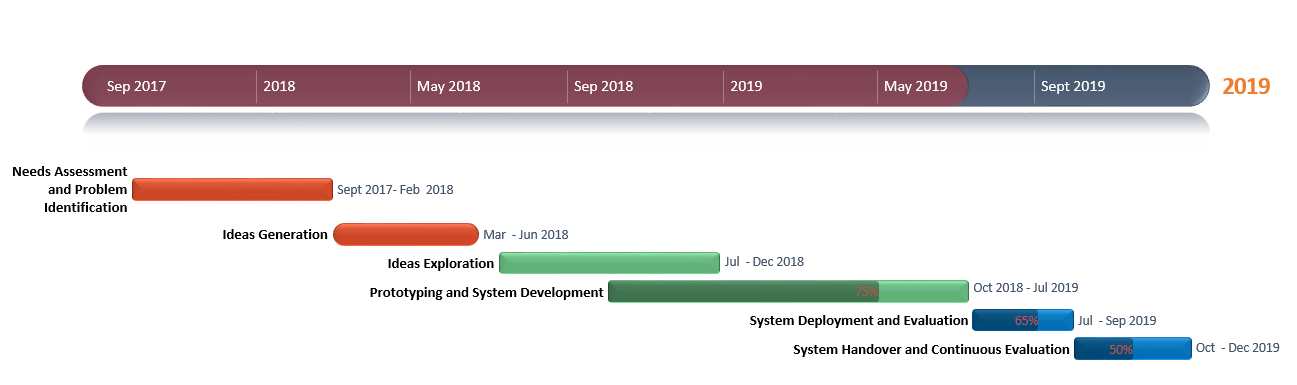
\includegraphics[width=17cm, height=10cm]{Figures/save.PNG}
    \caption{Overview of the 28-Month Study.}
    \label{fig:timeline}
    \end{figure}

 \section{Methodological Challenges in NICU Context}
 Throughout the co-design process, we encountered four co-design dynamics namely 1. power dynamic 2. shyness and fear 3. conflicts and disagreements and 4. group thinking (discussed in detail in the next three chapters) which affected the co-design process. To mitigate these dynamics and foster relationship between participants, we opted to use generative techniques such as incomplete sentences, emoticons, contextual map, role-playing, braindumping and scenarios to encourage all participants to voice their design decisions and engage in the discussion. 
 
 Although the co-design dynamics were not eliminated immediately, the use of mediated interaction approach through the generative design techniques helped the participants to gradually collaborate and work towards the common goal which was to design a tool that could enhance NICU communication. During the design process, I was able to build a deeper and more longitudinal understanding of the methodological considerations especially while working with multiple stakeholders in a sensitive NICU context. I realized that as a researcher, I need to have a list of several participatory methods---which I refer as "\textbf{basket of methods}"---that need to be modified, localized and paired before use to explore and achieve desirable outcomes. Methods  alteration and localization is necessary in sensitive context to ensure they align with the participant's cultural norms and environment.
 
 As a researcher undertaking qualitative research on sensitive topics, I learned the importance of assessing the impact of the research on the participants and myself. In this study, I faced many challenges including developing friendships, working relationships, emotional and physical safety, and conflict over roles. Most of the time, I neglected the negative effect that the study had on me and focused on ensuring that my participants were safe. I understood I was entering the lives of my participants at a time of stress and I focused on reducing any chance that could exacerbate their level of stress. However, this process made me feel uneasy about the level of disclosure during the interview sessions. At some instance, I got emotional and I had to divert the discussion to hide my emotions from the participants. This provided an opportunity for mothers to ask me unexpected questions about my personal life. Although I was not prepared for the self-disclosure, I felt like this opportunity was an important part of rapport-building process and I opted to use it to put myself on a level playing field with the participants.
 
  In addition, as a Kenyan computer scientist conducting research in South Africa, I encountered language barrier which hindered my interaction with participants during the co-design process. Some participants were hesitant to open up to me in recognition that my accent was different from the common South Africa accents. This was even worse when I arranged for follow up meetings in mothers' homes. They did not invite me to their homes due to security issues (i.e if a foreigner or visitor goes to their home, they become a target to the community gangs) but instead, they suggested we meet in public hospitals or police station. To build trust and enhance engagement in this study, I explicitly discuss the benefit of the research with participants (mothers and NICU staff) before delving into the data collection process. In some instance, I had to modify the research design to fit into the culture and beliefs of the participants.
 
\subsection{Working With Multiple Stakeholders}
Co-design is recognized as a methodology that supports inclusive problem solving and solutions finding~\citep{Jones2008b}. It places multiple stakeholders with disparate real life experiences and skills/knowledge to spend quality time mapping their journeys, identifying problems and developing possible solution that could mitigate the identified obstacles. However, this process is complex among multiple stakeholders because it increases the diversification through the the broadness of information, knowledge and suggestions of possible solutions. In this study, these differences led to co-design dynamics such as power dynamic, conflicts and group thinking which hindered collaboration. The hierarchical infant care structure in the NICU made the doctors and nurses to dominate the design dialogue thus limiting the mothers from sharing their design views. 

Attempt to counter these co-design dynamics and build relationship and trust among stakeholders demanded the use creative design approaches such as modification of methods, pairing of several methods etc. to encourage new ways of thinking that fostered collaboration among stakeholders. My methodological choices drew from literature in maternal and child care health, human-computer interaction for Development (HCI4D), psychology and Information Communication and Technology for Development (ICT4D). Although my experience and knowledge in health and psychology is limited, I occasionally use the basic knowledge gained through the online courses that I pursued to identify potential problems that commonly arise with various methods in these fields. 

Methodological considerations thus made from these multidisciplinary fields made my solution exploration approach more of a "trial and error". This approach although challenging, helped me learn that methodological solution in such sensitive interdisciplinary studies are not achieved immediately as one would expect. Instead, it takes time and effort to understand the environment and the people to ensure that the co-design process empowered the stakeholders to articulate the needs that they want to jointly meet with the researchers/designers.

For instance, I spoke to different groups of stakeholders (nurses, doctors, mothers, NICU supervisors) who had different needs with some of them not aligned with our research objectives. They all wanted the study to focus on their group specific communication needs so as to make their infant care role easy. Holding separate stakeholders focus groups, made me become aware of the broad and specific interest and goals of each group.  However, it was impossible to meet "everyone's" needs and requirements. Rather, I decided to have joint focus group with multiple stakeholders encouraging them to negotiate their disparate requirements. Based on their different NICU experiences, they were able to interact and cooperate constructively with each other in such a way that their different goals were addressed simultaneously.

\subsection{Understanding the Self in Conflict and Emotional Situations}
There were several instances when conflicts and disagreement arose during the design process. This depicted the hierarchical working relationship in the unit that hindered effective communication. As a researcher, this created an awkward design environment which I had no experience on. Hence, I opted not to interject the discussion but instead facilitate the sessions to ensure the discussion led to a constructive argument that would help participants to articulate their needs and technology desires.~\textcite{Rogers2013} insist that HCI researchers should focus on facilitating the design process and refrain from helping or engaging in the design process a discourse they refer to rhetoric of engagement. To adhere to this discourse, I chose to remain as researcher and put my effort in exploring different methods to encourage collaboration and enable participants to reach to a consensus. This helped me to understand the different perspective of participants, enabling me to see design ideas through their lens and learn why they are pushing back on other participants' ideas. 

\subsection{Emotional Effects on the Researcher} 
In the initial stages of this research, I experienced emotional difficulties as I conducted interviews to understand the NICU experiences and challenges  from the participants. The life experiences shared by participants---especially the mothers; were sad and had emotional toll on both the participants and myself. In such instances,  I evaded these emotional instances by diverting the discussion to a general talk such as baby's feeds and development to ensure that the participants and myself were emotionally stable by the end of the session. Also, I chose to play around with the children using the colourful audio picture books given to the mothers as a honorarium. Although these were temporary solutions, the interjection positively changed mothers' mood as they watched their children enjoy playing with the audio picture book. 

In cases where mothers needed further counseling services, I made arrangements with the nurses in the hospital who offered the needed support.  These emotional scenarios helped me to learn the importance of having counseling knowledge or skills as a researcher especially while engaging with vulnerable participants. In addition, I learned that researchers should have a flexible research plan that allows them to navigate ethics in cases where ethics in practice reveal new ethical dimensions. These ethics challenges in co-design research provides opportunities for consideration and improvement especially in HCI research ethics review processes.

\subsection{Considering Self-Care in Emotionally Demanding Research}
Prior to this study, I pursued online courses to help me to understand the sensitivity of this research and identify participants in case they were emotionally disturbed. Despite this preparation, I did not have access to information that could support me handle emotions as a researcher. As a result, I found myself engulfed with emotions as I engaged with participants during the problem identification phase. I did not pay attention to my emotions but instead focused on ensuring that participants emotional status was stable. I was not doing justice to myself and I would advise researchers conducting research in such sensitive settings to consider their physical and mental well being as they aspire to ensure that the research does not harm the participants. 
 
This consideration should be given a thought at the inception of the research. I learned the importance of providing practical suggestions while seeking ethical approval from Institutional Review  Board (IRB). I should have ensured that the ethics application protected both the participants and myself as I focus on achieving the stipulated  ethics. Instead, I upheld a naïve view of what such sensitive research studies and participants' collaborations require in terms of time and resources. As a result, planning and adhering to the approved  research ethics was challenging and I had to navigate the ethics as I focus on the  safety of the participants in order to achieve the research objectives.

\subsection{Methodological Consideration in Emotionally Charged Environment}
Base on the knowledge I acquired from the online courses, I was able to select methods that considered the sensitivity of the topic ensuring that the psychological aspect of the participants was protected. This was achieved by encouraging mutual learning concept during the design process to ensure the participants---especially the mothers, benefited from the exchange of the information. In addition, I learned the importance of focusing on taking precautions to reduce the effects of study on the participants by adopting suitable strategies such as duration and intensity of interviews, choice of question etc. Following these reflections, I recommend HCI researchers to focus on using research methods as a means to establish a relation of trust, because proximity and familiarity with the participants facilitates mutual knowledge. This is the only way to get oneself accepted thanks to a gradual entry that helps to minimise the social distance.

Through out the study, I sought to understand the impact and effect of the methodological decision I made as a researcher. Indeed the process has numerous pitfall which we drew lessons from. I learned that as a researcher engaging with participants in co-design to create supportive technological interventions, I need to be mindful of what I can offer ensuring that I do not impose my needs on them. Instead, I should leave the appropriation and innovation of technologies to the users of the technologies. \textcite{Taylor2011} findings reinforce my sentiment by arguing that HCI researchers should not frame and solve issues based on their theories rather they should provide practical tools that support engagement and new ways of learning to the participants. In that respect, we put our focus on methods that would enhance participants relationship ensuring that the hierarchical structure in the unit did not hinder some participants from voicing their design ideas. This was achieved by using paired methods in phased co-design approach. 

\section{Chapter Summary}





% This just dumps some pseudolatin in so you can see some text in place.
%\blindtext

  % Chapter 4

\chapter{Needs Assessment and Problem Identification } % Main chapter title

\label{Chapter4} % For referencing the chapter elsewhere, use \ref{Chapter4} 

%------------------------------------------------------

\section{Introduction}
In this chapter, we present a contextual inquiry study conducted with mothers of premature infants and Neonatal Intensive Care Unit (NICU) staff (doctors and nurses) at the Groote Schuur Hospital in Cape Town.  The goals of this study were to:
\begin{enumerate}
      \item Observe and familiarize with the NICU environment
       \item Establish a working relationship with mothers and NICU staff
        \item Identify stakeholders' NICU experiences and main challenges that hinders communication in the NICU; and
         \item Understand stakeholder's needs and requirement regarding a  possible solutions that could be used to enhance communication between NICU staff and mothers 
\end{enumerate}

\section{Research Perspective}
In this study, we chose to use a bottom-up user-centric approach \citep{Abras2004, Balaam2015} focusing on conceptualizing the NICU environment to understand the existing workflow, communication problems and design of a possible communication intervention. In this phase, we did not approach the NICU stakeholders with a specific system ideas. Instead, we motivated the stakeholders (nurses, doctors and mothers) to share the challenges they face while taking care of the hospitalized infants and provide suggestions of possible interventions that fit in their socio-economic situation.

We chose to use this approach because it focuses on the explicit understanding of users, tasks, and environments in which they work from~\citep{Abras2004}. In addition, this approach is encouraged health field because it agrees with healthcare institutions/organizations such as the National Academy of Medicine (NAM)\footnote{The National Academy of Medicine (NAM) is one of three academies that make up the National Academies of Sciences, Engineering, and Medicine (the National Academies) in the United States} that advocates for user-centric approach when developing healthcare technologies ~\citep{DeVitoDabbs2009}.  Furthermore, several researchers conducting Information and Communication Technology for Development (ICT4D) projects recommend this approach to improve quality and sustainability of technological solution~\citep{Heeks2008,Pankomera2018, Mukisa2017}.

\textcite{Piper2018} and ~\textcite{Rogers2013} sensitive the importance of understanding the stakeholders context and needs to ensure the designed tool meets the end users needs. However, most healthcare systems designed for developing countries often rely on top-down approach. The ICT4D and Human Computer Interaction for Development (HCI4D) researchers frame the needs of end users with their own theories and ordering and later impose them on the participants. Consequently, this increases the researchers' tendency to designing and developing technological solutions based on their own understanding. ~\textcite{Rogers2013} refers to this approach as designing in "third-person mode". This is a case where the researcher has predefined research needs and goals, therefore imposing them on the participants during the design process. Often, this design process ends up with easy-to-use systems that are usually used in the inception of the system deployment but later the users stop using them.

In the design of health care systems, patients or caregivers involvement: where they share their lived experiences of health and social care; is essential to ensure that the researchers understand not only their system desires but also their feelings and needs. In addition, it help the researcher to utilize patients or caregivers specialist knowledge which in return gives participants a strong voice in how health systems or services should change. This last aspect is essential if changes are to be sustainable in healthcare. Furthermore, previous studies have proved that such participation allows the researcher to build a rapport with the participants which is more important than the designing a system which end users might not relate to \citep{Wolstenholme2017,Nilsson2016,Ward2018}. 

In the same vein, this study focuses on engaging the participants throughout the design process to empower and encourage them to articulate their design needs and ideas. We acknowledge that our stakeholders have limited prior design skills but based on their rich lived NICU experience, they were best placed to design the appropriate technological artifact that could bridge the communication gap in the NICU. On that basis, we did not approach our stakeholders with a defined design idea. Instead we allowed them to lead the co-design process and explore possible technological solution according to the technologies they possessed or had access to. This approach empowered participants to fully engage in the design process, encouraging them to contribute towards the shaping of new technological intervention that could meet their needs in their existing socio-economical condition. We argue that this approach progressively fostered mutual learning  between multiple stakeholders in a hierarchical infant care structure, enabling them to collaborate in identifying most viable technologies that could be used in Groote Schuur Hopital (GSH) NICU context.

In the sections that follow, we discuss the methods used to understand the NICU environment and stakeholders, what we learned and the outcomes of our activities concerning the design of the a possible communication intervention. Since we have not come across existing literature that focus on design on NICU systems in low-income context, we argue that our methodology approach helped us to familiarize and understand the stress related to premature birth and the communication challenges that the NICU staff and mothers face as they partake in the care of the hospitalized infants.

\section{Needs Assessment (Sept 2017- Feb 2018}
The focus  of this phase was to introduce the study to the stakeholders (mothers of premature infants, NICU nurses and doctors), engage them in identifying the common NICU communication challenges and suggestions of possible solution that could solve the NICU communication issue. This research was conducted at Groote Schuur Hospital (GSH) Neonatal Intensive Care Unit (NICU), a state-funded tertiary referral center for sick and preterm infants in Cape Town \citep{WesternCapeGovernment2014}. GSH serves the predominantly indigent sections of the Cape Town population. The 75-bed capacity neonatal unit admits approximately 2000 infants annually, 500 of which are preterm infants with a birth weight less than 1500g \citep{Kapembwa2017}. The infants admitted in this intensive care unit are largely from poor socioeconomic backgrounds~ \citep{Thompson1993}. 

We used observation and semi-structured interviews research methods to engage with the NICU stakeholders and also to ensure triangulation of data. Before commencing with the data collection process, we applied and received ethics clearance from University of Cape Town, Faculty of health science ethics review board in September 2017. We discussed the research objectives with all our participants and asked them to voluntarily sign the consent form before engaging in data collection process with them. The data collected was safely stored by the researcher to maintain participants confidentiality and anonymity. Next, we discuss the data collection process.

We Recruited the staff from different sections of the NICU to understand the communication challenges in the unit and to gather their perceptions and opinions on the use of technology to support communication in the NICU. Instead of working with both parents of the premature infants, we opted to work with mothers who were 18 years and above. We arrived at this decision based on the initial visit we conducted at the hospital. Our contact person, who is currently a neonatologist at the unit for over five years mentioned that most mothers are not married and they solely care for the infants and other children at home.To avoid participants discrimination during recruitment based on their marriage status or better said to avoid the unmarried women from feeling less inferior while interacting with other married couple, we agreed to leave out the fathers and only include them during the evaluation process.

Also, according to ~\textcite{Waycott2015}, it is important for researchers to communally reflect on ethical encounters while conducting research in sensitive settings such as the NICU to ensure that the study does not exacerbate stress among participants. To uphold this ethical practice, we chose to work with mothers of infants who had been discharged from the NICU for at least three months to ensure the stability of the infants’ health and the emotion status of the mothers.

\subsection{Observation}
We conducted observation in two parts. In the first part, I volunteered to work in the NICU and help the nurses to conduct duties such as infants cup feeding and cleaning, that do not require medical expertise. We also supported mothers in the unit who requested for our assistance. The main aim of the volunteer work was to familiarize with the NICU environment and built trust and working relationship with the staff. In the second part, I visited the NICU and observed NICU activities and workflow in all sections of the NICU both during the day and night for at least one hour per session. The objective of these observation sessions was to understand NICU workflow and communication challenges in totality. In the next sub-section, we discuss in detail the  the observation sessions activities.

\subsubsection{Volunteer Work at the NICU}
After receiving the ethical clearance, we registered with GSH benevolence department to work as volunteer at the NICU. \textcite{Ross2014} states that most Human Computer Interaction (HCI) conducting participants observation do not interact or involve wit the activities of the participants. Instead, they choose to remain as outsiders where they observe participants from a distance as they take their notes. To overcome this limitation in our study, we chose to volunteer at the NICU so that we familiarize with the NICU environment and activities such as: what happens at certain time in the unit, who does what, how do NICU staff relay information to the mothers, what are current communication mode and so on.

The NICU has five sections, namely; Intensive Care Unit one (ICU1), ICU2, High Care one (HC1), HC2 and Kangaroo Mother Care (KMC) sections. For the volunteer work, we were allocated at KMC; a section that admits infants whose health is stable and are being monitored before they are discharged. The neonatologist introduced us to the nurses and asked them to collaborate with us as we work in the section. For three months, we worked in the section once a week for at least 3 hours. During this period, we cup feed and cleaned the infants as per the instructions given by the nurses. We also helped the mothers to dress their infants, fetch breast milk from the fridge and also supported them as they conducted skin to skin care; a method of caring for new infants that is commonly referred to Kangaroo Mother Care (KMC). 

This opportunity helped us to familiarize wit the NICU environment and identify some of the communication challenges that NICU staff and mothers encounter as they take care of the hospitalized premature infants. Most mothers are stress due to lack of timely communication wit the NICU staff. To deepen our understanding on the communication challenges in the NICU, we opted to conduct observations in all sections of the unit.

 \subsubsection{Observation in All Sections of the NICU}
As  noted  by~\textcite{Millen2000f},  rapid ethnography  is  essential to  understand  the  people and context of use for the designed technological intervention. To deepen our understanding on NICU environment and the people, we  meet the NICU nurse supervisor and her assistant and scheduled the observation sessions.Later, we taken around the unit and introduced to the nurses in all sections of the NICU. We also attended the doctors' weekly meeting where we our NICU contact person shared our research objective and asked the doctors to collaborate with us as we work in the NICU. This exercise was essential, especially in the NICU to ensure that the NICU staff knew my objective in the NICU environment which is strictly  restricted for the infant family visits.

In one month, we conducted observations in all sections of the NICU and each observation session lasted approximately 45-60 minutes. We visited the NICU session in different time of the day--- in the morning, during the day and at night to gather comprehensive understanding of the NICU activities and identify distinctive workflow at different times of the day. Specifically, we observed the NICU interactions (between doctors and nurses, NICU staff and mothers and among mothers), NICU staff daily roles, communication challenges and technologies used to enhance communication in the unit. 

Field notes were recorded during all observations to maintain the richness of the data. These sessions generated additional information that strengthened and triangulated the validity of the findings identified during the volunteer work period. As a result, this expanded our ability to contextualize and make sense of the NICU environment and workflow. 

\subsubsection{Semi-Structured Interviews with Participants}
After conducting observations for four months, we decided to conduct one-on-one interviews. The aim of these interviews was to verify and develop a comprehensive understanding of the information collected during the observation sessions.  We recruited 10 nurses (those working during night and day shift) and 5 doctors from the NICU. The staff were selected based on the fact that they had worked in the NICU for more than six months. The supervising nurse at the NICU gave us a list of mothers who had infant developmental check up appointment scheduled in the month of February 2017. We called the mothers prior to their clinic appointment to remind them of the scheduled infant check up as well as to introduce ourselves before meeting them. 

These  appointments happen at at Mowbray hospital \footnote{Secondary level referral hospital treating women with complicated pregnancies who are referred from the Midwife Obstetric Units (MOU) in  the metro west area of Cape Town.}. This government hospital has a clinic that focus on monitoring the development progress of premature infants who have been discharged from GSH. The clinic is opened on Wednesday from 8 a.m to 12 noon. We visited the clinic every Wednesday morning to recruit mothers for interview sessions. The doctor in charge of the clinic introduced us to the mothers who were seated at the bay waiting to be attended. We approached the mothers and briefed them on our study objectives before requesting them to voluntarily participate in one-on-one interviews. Prior to the interviews, we volunteered to dress and play with infants after their weight was taken while awaiting to be attended by a doctor for further checkup. 


Over a period of four weeks, we managed to recruit 15 mothers (3-4 mothers per week) of preterm infants whose infants had been discharged from the hospital for at least three months. This was a precaution in ensuring the health of the infants and their mothers’emotional status was stable. After attending their infants' appointments, we ushered the mothers to a private room that the hospital provided for us to conduct confidential interviews. To warrant anonymity of participants, photos were not taken during these sessions. However, we audio recorded conversations and took field notes on participant's approval.  This being a qualitative research, we choose to use this sample size (15 NICU staff and 15 mothers) after attaining the saturation. In qualitative research, saturation is attained at the point where collecting additional data will yield similar responses to those obtained earlier thus further data collection is not required \citep{morse2000, Malterud2016}. 

In line with \textcite{Glaser1967}, we recommend saturation as a methodological principle and criterion for achieving an appropriate sample size while conducting qualitative studies. We used open-ended interview questions to encourage participants to provide additional information, including feelings, attitude and their understanding of the research objectives. We opted to prioritize interviews with NICU staff before engaging mothers. This approach was adopted because we had initially built trust with  staff during the observation sessions. In addition,staff were readily available in the NICU unlike the mothers who were only available during infants' clinical check ups. Also, we were of the opinion that prior engagement with NICU staff would help us understand  NICU melieu in totality making it easier for us to subsequently interact with mothers who were only in the unit for few a days or months. 

During the interview sessions, we  focused  on understanding  the  main challenges that hinder effective communication between mothers and NICU staff. In addition, we sought their perception on the use of technology to improve communication in the NICU. Mothers had to sign a consent form before the interview sessions and we guaranteed them  the confidentiality of the information provided. The interview sessions took an emotional toll on the researcher and in some instance, we had to divert the interview to a general topic before resuming with the interview. Playing with the children was a good way of taking a break. Through this activity, the researcher was able to create a bond with the mothers. As a honorarium,we gave each mother a picture book to compensate them for the interview time taken. We opted to give them these books because they help to improve children brain development. In the next section, we discuss the findings from our observation and interview sessions.

\section{Data Analysis}
We transcribed all the data collected during the observation and interview sessions and included the non- verbal expression in our final transcripts. We used Nvivo software to analyze the qualitative data subjecting it to a three-stage analysis method: data reduction, data display and conclusion drawing (Bottoman, 2004), (Pini, 2012). Open coding (Glaser and Strauss, 1967) was used to look for recurring themes in the data. We choose to use “grounded theory” to develop an understanding of social phenomena in NICU environment and ‘discovered’ or generated concept from the qualitative data collected (Lawrence and Tar, 2013). From our data, we came up with four themes that represented participants feedback. Using Nvivo we could easily identify the relationships between themes and figure out underlying ideas and meanings among them.

In the next section, we present these research themes; in particular, we reveal the current workflow in the NICU, the communication challenges, use of technological interventions and  perception of our participants towards the use of technology to enhance communication in the NICU.

\section{Observations and Interviews Outcomes}
The diagram below provides an overview of the NICU workflow that we identified during the observation sessions.
\begin{figure}[htp]
    \centering
    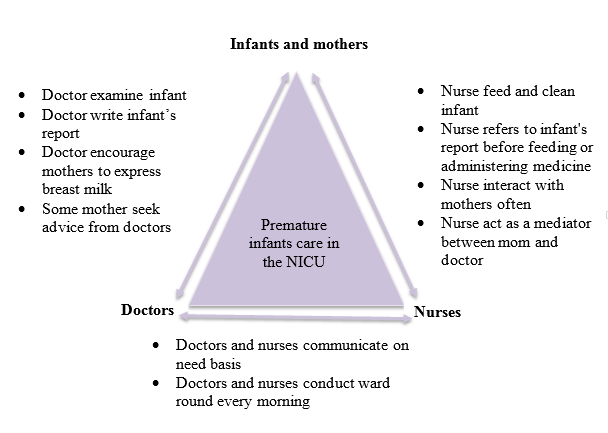
\includegraphics[width=15cm, height=10cm]{Figures/workflow.PNG}
    \caption{Groote Schuur Hospital NICU Workflow.}
    \label{fig:workflow}
    \end{figure}

We identified that the infants are fed in four-hour intervals, a schedule that nurses adhere to ensure that the health of the infants improve. The nurses use the feeding and medication instructions issued by the doctors. While conducting our volunteer work, nurses informed us that breastfeeding is critical to premature infants’ recovery and mothers are sensitized to express enough milk for their infants~\citep{Kapembwa2017, Updegrove2013}. Without this, infants fed on formula milk are at the risk of developing Necrotizing Enterocolitis (NEC); a disease that affects the intestine of premature infants in the second to third week of their life ~\citep{Updegrove2013}. 

We recognised that communication is essential while taking care of premature infants. Doctors and nurses interact often when conducting medical procedures on infants in the ward to ensure that they are in the same page in terms of the infants' condition and the treatment. Nurses consult the doctors before administering medication or discharging/moving an infant from the unit. On the other hand, doctors consult each other often and sometimes they use the neonatal medical book or use their phone to access online medical information when conducting procedures and writing medical reports.  

However,there is minimal communication between the NICU staff and mothers of premature infants.  A number of researchers have documented this finding ~\citep{Griffin1998, Pascoe2016, Jones2015}. From our observation and interview sections we identified that the nurses interact with mothers only when training them on latching and skin to skin care. The main reason for these minimal interactions is because the NICU staff are constrained by a heavy workload. As a result, they rarely interact with mothers to offer psychological support. This finding resonates with prior studies that  reveal that  mothers are prone to stress due to lack of regular and informative communication with the NICU staff ~\citep{Orzalesi2011,HadianShirazi2015, VandeVijver2015}. This was one of the motivation that made us focus on understanding the essential information that mothers need so that they can understand their infants’ condition and health progress. To further investigate the needs of the mothers, we opted to observe all the sections in the unit both during the day and night.  

\subsection{NICU Environment}
Groote Schuur Hospital NICU is equipped with incubators, monitors and other machines that are used to care for sick premature infants. The unit is small with incubators placed close to each other with plastic seats in between the incubators. To prevent overcrowding, the unit restricts visits to parents and grandparents of sick infants. However, during interview sessions, mothers mentioned that they would appreciate if visitors---especially their spiritual leaders, were permitted to visit and conduct prayers for their hospitalized infants. To clarify why such visits are discouraged, one nurse shared the following anecdote:

\enquote{\itshape We once had an incident where a spiritual leader applied oil on the infants face which is not allowed because infants' skin is sensitive. The same oil could be a potential source for spreading germs because of its application on other users outside the NICU}. 

During the day, doctors and nurses conduct rounds in the unit at around 11 a.m. Doctors have a responsibility of providing medical reports of all infants under their care. Their discussion happens around infants' incubators and mothers are seldom included in these discussions. One mother mentioned:
\enquote{\itshape The doctors would only ask me how I am doing and continue with their conversation like i was not there.}
NICU staff revealed that language barrier is the main hindrance to mothers engagement in these discussions. To affirm this claim, majority of the mothers said they could not understand the accent of the doctors and they required nurses assistance to interpret the information on infants' progress report book. In addition, technical medical terms are often used and mothers barely understand them. Instead, mothers usually nod in agreement despite not understanding what the NICU staff are talking about.

At night, there are few mothers in the NICU. Mothers and their partners are allowed in the unit until 8 p.m. There are few nurses at night and they work round the clock to ensure infants are fed and cleaned on time. Only one doctor is on call to handle emergency cases. Both doctors and nurses conduct rounds in the unit to ensure NICU equipment connected to the infants are operational. Next, we provide and discuss detailed activities of each section in the unit. 

\textbf{ICU1 Section:} ICU1 admits critically ill infants who are referred from other hospitals in Cape Town or newborns from the GSH labor ward. These infants are always under supervision to ensure that they breathe normally through the support of machines. Doctors in this section work closely with the nurses to confirm the infants receive the correct amount of oxygen and medication. There are few mothers in this section. Reason being majority of them are still recovering in the obstetric ward and are not able to frequently visit the section. 

The admitted infants are tiny and their sight is traumatizing. Mothers mentioned that they were uncertain of their infants' survival based on their small size and weight. They relied heavily on NICU staff to support them during this challenging times. Similarly, the sight of the infants had the same effect on the researcher. As acknowledged by (Moncur, 2013), it is important for researchers conducting sensitive study to have support mechanisms in case they become distressed or troubled by their research. To adhere with this practice, we sought psychological support from the senior nurses at the unit who oriented us to the section daily activities such as minor operations, blood transfusion and occasionally resuscitation. This helped us to understand and familiarize ourselves with the workflow and activities of this section. The nurses also advised us to focus on other sections since we were not comfortable with the intense medical activities in ICU1. We only spent three days in this section and focused on other sections as advised by the nurse.

\textbf{ICU2 section}: The ICU2 section is located opposite the ICU1 section. In between these two sections, is the working station where nurses and doctors handle NICU related phone calls. Similar to ICU1, this section admits critically ill infants whose breathing is supported by machines. Contrary to ICU1 section, in ICU2, there is presence of mothers accompanied by their partners who offer them support as they strive to adapt to the NICU environment and motherhood in general. Majority of these mothers remain admitted in the obstetric ward and they visit this section to deliver their expressed breast milk. They seemed to be in pain and as they were still recovering from cesarean childbirth. Also, we observed that most mothers struggle with breast milk expression and occasionally they requested for nurses assistance. Due to nurses heavy workload, they handed over pamphlets to mothers and asked them to learn milk expression from the instruction provided. Due to insufficient support, these mothers sit next to their infants’ incubator and cry as they attempt to express enough breast milk for their sick infants. During interviews sessions, mothers confirmed they were distressed by the sight of their infants connected to numerous devices and cables, for which they did not understand their functions. 

In addition, they mentioned that the NICU environment in general was terrifying. This confirms \textcite{Obeidat2009} claim that NICU environment is intimidating thus causing significant level of stress on mothers. Mothers mentioned they are afraid of touching their infants lest they disconnect the cable attached to them. In addition, the alarms of the display machine connected to the infants kept going off, thus agitating new mothers in the section. At one instant, we saw a mother calling out the nurses when the alarm connected to her child's display machine started blinking. The nurse switched off the alarm without informing the mother what triggered the alarm. The nurse checked the infant and told the mother that everything was fine with the infant. When the alarm went off the second time, the same mother switched off the alarm without consulting the NICU staff. This was common among mothers in this section. The nurses informed us that the alarm sometimes are triggered by frequent touching of infants which interferes with infants' thermal regulation. This case is not critical, though they mentioned that the machine calibration needed to be reset to fix some of the false alarms. The nurses' remarks thus explained why we observed fewer alarms at night.

 \textbf{High care 1 and high care 2 sections:} The High care 1 and high care 2 sections admit infants with chronic illness. These infants can stay in these sections up to three months. There are numerous mothers during the day who visit the unit on a daily basis to nurse their infants. These mothers come in the morning with a jar of expressed breast milk. First thing, they label the jar with a sticker and store it in the refrigerator. Then, they sit next to their infants’ incubator and continue expressing more breast milk or they conduct skin to skin care. Mothers said they liked holding their infants in their arms to forge mother-infant bond. To encourage mother-infant bond, nurses inspired mothers to take up their maternal role by training them to cup feed, clean and hold their infants close to their skin. Although mothers were expected to visit the unit everyday, we noticed some mothers occasionally visited their infants. In cases where a mother did not visit the unit for two consecutive days, nurses used landline phone to ask them to deliver expressed milk to the hospital. Infants who were rarely visited were fed on formula milk, exposing them to gastrointestinal infections which has an effect of slowing their development \citep{Embleton2001}. \enquote{\itshape We always make an effort to educate mothers on the importance of breastfeeding}, said the nurses. They intervene by giving mothers pamphlets which list the benefits of breastfeeding. The pamphlets are usually in English, isiXhosa and Afrikaans language.

Despite nurses intervention, mothers who are new to the unit appear to be lonely. In one instance, a mother was seen calling out a nurse to help her with milk expression. The nurse gave her a pamphlet and asked her to follow the instructions before resuming on her busy schedule. The mother appeared frustrated because she was not able to express any milk despite following the instructions. \enquote{\itshape The NICU staff are always busy with minimal time to interact with us},mothers affirmed. As a result, mothers tend to consult each other. During our observation sessions, we viewed them trying to interpret the medical reports of their infants. They also shared their personal information and encouraged each other the best they could.

However, majority of mothers are afraid to approach the doctors. During the ward rounds, mothers tend to be more of observers and they seem not to understand their infants' development status. In one instance, a mother was asked whether she understood the condition of her infant. \enquote{\itshape I can not understand the medical terms contained in my infant’s progress report}, she said. The consultant asked one doctor to explain the condition in simple terms but eventually, the conversation ended up being complex thus leaving the mother out of the conversation. Eventually, mothers opt to follow up on the ward round conversation by approaching nurses who can communicate in their vernacular languages. In the case where nurse are not able to interpret medical information, they involved doctors in the conversation, as they act as information mediators. 

\textbf{Kangaroo Mother Care (KMC) section:}
The KMC section admits infants with stable health who awaits to be discharged. Mothers in this section are familiar with the NICU environment after being there for more than one month. However, there are new mothers in this section who need constant assistance from the NICU staff. There is staff shortage and only three nurses and one doctor are allocated in this section. These NICU staff are overwhelmed with the workload and we noted that infants cry longer before they are attended to. In some instances, we observed nurses giving syrup to crying infants to sooth them to sleep so that they could continue with their daily role. In addition, the alarms go off quite often and they remain unattended for a longer time than in other sections. 

There are few mothers in this section. This is because mothers are aware of their infants' stable health and they await to be discharged. Nurses confirmed this when they said:

\enquote{\itshape Mothers whose infants have been admitted in the NICU for a long time feel relieved when their infants are transferred to the KMC section. They are assured they will be going home soon}. 

Also, one mother mentioned:

\enquote{\itshape My child had breathing issues for two weeks. I got relieved when i found nurses had moved her to the KMC section}.\bigbreak

KMC is generally the last section an infant goes through on their path to recovery and discharge. Mothers visit the section only when they are delivering expressed milk for their infants. For mothers who are unable to commute frequently, the hospital has set aside a small room in this section where mothers can board.

Unlike in other section, mothers in this section were familiar with breast milk expression and conducting skin to skin care. They required minimal assistance from the nurses as they cared for their infants. These mothers have learned the habit of switching off alarm without consulting the NICU staff. Majority of mothers mentioned: \enquote{\itshape I saw other mothers switching off the alarm and I decided to do it as well.} Nurses are mostly busy and have no time to attend to the alarms. Instead, they focus more on infant feeding and hospital transfer or discharge planning. Due to lack of sufficient information, mothers are not equipped to engage in the decision making of their infants health and care of their infants. As a result they feel like they have lost their maternal role which often make them worried and anxious thus exacerbating their level of stress. In the next session we discuss factors that we identified as the major cause of stress among mothers of hospitalized premature infants.

\subsection{Source of Stress In the NICU}
Premature delivery and hospitalization are stressful events for mothers \citep{Wigert2012, Heidari2017}. Our stakeholders confirmed that NICU environment is stressful for everyone. Mothers mentioned that they didn't expect to deliver prematurely since they routinely attended antenatal appointments. Therefore their infants admission in the NICU was unexpected and traumatizing. All the same, five mothers (two were hypertensive and three diabetic) mentioned that doctors had prepared them psychologically and they were aware of possibilities of premature birth. From our interviews session we identified and categorized the common sources of premature relate birth stress into four groups as discussed below:

\subsubsection{Infant’s Health Condition}
The main cause of premature-related stress is the uncertainty of infants' health condition. All mothers mentioned that their infants health was unpredictable since infants' condition fluctuated quite often. For instance, one mother said:

\enquote{\itshape Each and every day, my child was on a different type of oxygen and I did not understand why his health was deteriorating} \bigbreak
Another mother mentioned:

\enquote{\itshape My babies weight was low and it was not improving. She vomited all the milk she took. She had to be moved from Highcare1 to ICU2 section. This was stressing. I expressed enough milk for my baby but her health was not improving} \bigbreak
Mothers relied heavily on the support they received from NICU staff to manage their levels of stress. However, NICU staff have minimal time  in their schedule to provide psychological support to mothers. In stead they work round the clock to ensure that the infants are fed and cleaned. On the other hand, mothers are unable to understand the medical terms used when NICU staff share infants' health update with them. To handle this challenge some mothers, opt to befriend nurses who speak their vernacular language to receive frequent updates on their infants' health status. Foreign mothers and those who are unable to speak South Africa common languages always feel out of place and helpless.
 
\subsubsection{Economic Factors}
Mothers whose infants are admitted to GSH NICU are mostly from low-income communities around Cape Town. Majority of them are single parents and they receive support from their parents and the South Africa government social funds. All of them encountered financial challenges during their infants hospitalization. \textcite{Blencowe2013} review of epidemiology of preterm birth shows that the cost related to neonatal intensive care are high and they place additional burden on families resources. We confirmed this finding as we interacted with mothers who participated in this study. They mentioned that they incurred high high transport cost---which they had not budgeted for, whenever they travel to the hospital.

\enquote{\itshape I had not budgeted for the travel cost and i used a lot of my saving on taxis. I had to skip hospital visits whenever  i did not have money, although I did not feel comfortable being away from my child} \bigbreak
We also identified that three mothers had to quit their job to take care of their hospitalized infants. They were not entitled to maternity leave thus leaving them with no option but to quit their jobs. Consequently, they encountered financial challenges which affected them emotionally because they could not provide basic needs to their families. One mother commented :

\enquote{\itshape I had other children back at home and I was torn between taking care of the family back at home and visiting the sick child in the NICU.}

\subsubsection{Social-Cultural factors}
11 out of 15 mothers related their premature birth and hospitalization to their various cultural beliefs. Separation and reduced opportunities to interact with their infants are against their culture and they felt they were not fulfilling their maternal role. Also, they attribute their premature birth to certain cultural practices they failed to conform with while pregnant. For instance, one Xhosa woman said:
\enquote{\itshape I didn't follow the Xhosa cultural practice when I was pregnant and I sometimes think that's what caused the early birth. In my culture, we must follow the cultural practice to prevent evil spirits from attacking the fetus.}
 In addition, religion and spiritual practices, served as a background to explain the present condition of their infants. These sample of comments expresses mothers views:
 
\enquote{\itshape I believed that my child would get well if the Imam prayed for him. Unfortunately, the Imam was only available at night and the NICU would not allow visitors past 8 p.m. I was depressed and I felt like my child's health was deteriorating because we did not conduct the prayers.} 

\enquote{\itshape I believed that if my pastor anointed my child, he would have gotten better quicker}
From the interviews, we identified that mothers incorporated their cultural beliefs while providing care to their infants. We comforted the mothers by educating them on possible causes of preterm births. We also informed them that preterm birth can happen to anyone and it is not related to any cultural practices. To reiterate on this information we asked mothers to further consult clinical information pertaining causes of preterm births from nurses who were familiar to their cultural practice.

\subsubsection{Insufficient Communication} 
Lack of supportive and up to date neonatal information emerged as the major cause of stress among mothers of preterm infants. 13 mothers, felt like the nurses had taken up their parental role and they were not involved in their infants' health decision making process. For instance, one mother said:

\enquote{\itshape I was admitted to the obstetric unit and when I went to visit my baby in the NICU, I found my child being fed with formula milk. I was angry because no one had asked me for my breast milk} \bigbreak
Another mother mentioned:

\enquote{\itshape My child was moved from ICU2 to high care1 section and I was not informed. I had to walk in the NICU thinking the worst had happened to my child but I later found her.} \bigbreak

They mentioned that they needed emotional support from the NICU staff to help them cope with their infants, illness and other aspects of the NICU environment. Akin to \citep{Axelin2006} study, mothers wanted detailed information of the NICU procedures that staff conducted on their infants to help them manage the stress related to painful situations of their infants. Two mothers mentioned that they say doctors drawing blood from their infants' and they could not stand the sights because their infants were crying loudly.

\enquote{\itshape They did not tell me what they were doing to my child and I felt helpless because I could not protect him from pain}\bigbreak

\enquote{\itshape My baby cried a lot when they drew blood from her head. They did not tell me what the test was all about and I felt helpless not knowing how to comfort my baby.}\bigbreak

We followed up with the doctors to understand why they did not involve mothers during NICU procedures.


\enquote{\itshape We do not encourage mothers to be around the procedure table because the process is intensive and they always get overwhelmed with emotion thus interfering with the process}\bigbreak


\enquote{\itshape We use simple language to inform mothers about the procedures but they seem not to understand. }\bigbreak
Also, mothers mentioned that the NICU environment is filled with unfamiliar equipment which they are never oriented on once their infants are admitted in the NICU. They fear touching their infants lest they disconnect cables connected to them. In addition, the alarms in the NICU keep going off and mothers are not sure what triggered them. They reiterated that it was important to be oriented to the NICU environment and equipment to help them familiarize with the environment. 


Based on these responses, we concluded that there is communication barrier between staff and mothers. Similar results were reported by \citep{Mok2006, Aagaard2008}. Ineffective communication between staff and mothers strains their cooperation in infant care thus aggravating mothers stress levels. Mothers want frequent communication with staff which included chats, encouragement and general talk about premature birth. However, NICU staff mentioned that the NICU has shortage of staff and they work round the clock to ensure that the infants health stabilizes thus neglecting the emotional needs of mothers. Consequently, mothers,struggle with sharing the care of their baby and in building strong relationships with NICU staff. They avoid voicing their issues in fear that this might make them appear as difficult mothers which in turn may stop the staff from tendering to their infants. To enable the reader to understand the communication challenges in the NICU, we will categorize NICU communication into three groups and discuss them in the next section.

\subsection{Communication in the NICU}
The care of premature infants involves different stakeholders who need frequent sharing and discussion of information related to infants' health status~\citep{Wigert2014b}. Effective communication among the NICU staff, and between the NICU staff and the parents is essential for informed decision making and parental satisfaction~\citep{Kowalski2006}. Based on our observation and interview sessions, we identified three categories of  NICU interaction. These are Communication between: 1. NICU staff 2. NICU staff and mothers and 3. mothers. 

\textbf{Communication between NICU Staff:}
The nurses, doctors and the NICU clerks work closely to ensure that they are in the same page in terms of infants health status. In the morning at 7 a.m when the day shift nurses report at work, they take a ward round with the night shift nurses who update them on the health status of each infant. Infant information is recorded in each infant's progress report book which is placed on a tray beneath the incubator. Similar communication happens in the evening at 7 pm when the night shift nurses arrive.

During the day, doctors and nurses conduct a ward round at 11 am. Doctors give a report of each infant’s health condition and progress to the team. At the same time, nurses take notes to record health condition of each infant. We identified that most of the communication during the ward round is between doctors. Nurses were only involved when they needed to specify the amount of feeds and medication administered on infants. Hence, we established that communication between doctors and nurses were few and they happened on need basis. During the day the main conversations between doctors and nurses is around the infant feeding, medication and hospital discharge/transfer information. Nurses consult doctors when they need clarification on feeding or medication information. During section transfer or hospital discharge, nurses must consult the doctor before the infant leaves the section.

Moreover, we identified doctors and nurses have separate reporting books and meetings which are held at different days of the week. Nonetheless, the doctors do invite nurses in their weekly meeting which is held every Friday at 11pm. During the day the main conversations between doctors and nurses is around the infant feeding, medication and hospital discharge/transfer information. Nurses consult doctors when they need clarification on feeding or medication information. During section transfer or hospital discharge, nurses must consult the doctor before the infant leaves the section. 

Nurses work together to ensure that the infants are fed and cleaned at the scheduled time. They consult each other before administering medication. For instance, we observed two nurses using a calculator on their mobile phone to calculate the drug dosage. On follow up, we learned that they use calculator to ensure infants receive the correct dosage to avoid further complication. To ensure smooth running of NICU workflow, they take tea and lunch break in intervals. Before a nurse leave the unit, they have to alert others so that all NICU sections are covered throughout the day.

On the other end, doctors interact among themselves when they are conducting procedures or when discussing infants’ health condition. They meet around infant incubators and discuss infant’s diagnosis. Although, they rarely include mothers in these conversation. Often, doctors work individually in their allocated part of the section.

\textbf{Communication between NICU staff and mothers:}
Communication between mothers and their infant’s principal medical care providers is important in the NICU setting. It ensures that mothers are involved in every decision made on their infants’ health \citep{Orzalesi2011, HadianShirazi2015}. It is important for mothers to freely communicate with staff in the NICU to understand their infant’s condition, participate in medical decision making and  partake in the care of their infants~\citep{Wigert2014b}. However, we identified there is minimal interactions between the staff and the mothers--- especially those between mothers and doctors. 

\enquote{\itshape We have a heavy workload and rarely have time to support or interact with mothers}, doctors confirmed. They are overwhelmed with their daily NICU duties thus leaving them with little time to interact with mothers.

Nurses often interacted with mothers who are new in the NICU to educate them on breast milk expression, cup feeding and skin to skin care. This initial interaction is brief and the nurses subsequently give mothers pamphlets to complement their interaction. Nonetheless, they follow up on mothers who face lactating challenges to educate them on breastfeeding diet. Also, they interact with surplus breast milk to encourage them to donate to the hospital milk bank that support infants whose mothers are not able to express enough breast milk. Although nurses strive to support mothers, they mentioned that some mothers do not comply with the advise provided. For instance, we observed a mother being scolded by a nurse because she had not delivered expressed milk for her baby. The nurse said:

\enquote{\itshape Your baby is sick and vomiting because you don’t want to express milk. Formula milk is not good for your baby and you are not putting any effort to help her}\bigbreak

Nurses said that they are sometimes demanded to be harsh on the mothers to ensure that they cooperate in infant care. As a result, mothers fear them and comply to their request to avoid being rebuked. 

For mothers who are concerned with their infants health status and development, NICU staff often prioritize on providing them with infants' up to date information. They use layman's language to explain infants' condition to mothers. Even so, some mothers are not able to understand medical information pertaining their infants. This is either because they fear asking questions or they do not understand English. The staff said infants health is unpredictable and they often provide mothers with accurate information to calm their anxiety. Although worrying and anxiety are sometimes unavoidable among mothers, doctors try their best to offer psychological support when needed. 

\enquote{ \itshape I pay close attention to maternal instincts. I believe mother-child's bond is strong and if a mother insists that I should check on her baby, I do it immediately because their intuition may be suggestive of child’s health condition}, disclosed a doctor. \bigbreak

Over all, there is minimal interaction between doctors and mothers in all sections of the unit. During the ward rounds, doctors initiate conversation with the mothers but they seem not to understand the shared information. Mothers often nod in agreement to everything said by doctors but when asked to explain their infants condition based on their understanding, they keep quiet or sometimes confirm that they do not understand the medical terms used. Most mothers are afraid to initiate a conversation with the doctors and they mainly rely on nurses to connect them with the doctors.

\textbf{Communication between mothers:}
Mothers interactions are common in HC1, HC2 and KMC sections. Majority of these mothers have been in the NICU for more than two weeks and they appear to be familiar with each other. They sit close to each other and chat about their infants' health and personal information. All mothers commended these interactions saying that they were supportive and necessary especially when a mother is new in the NICU. We established these mother-mother interactions played a  peer-support role as well as an encouragement channel for mothers in the NICU. One mother confirmed this when she said:

 \enquote{\itshape I talked to a mother who told me that her son had the same condition as my baby and he was fine after two weeks. This was encouraging and it helped me to stay positive}

Another mother who was new in Cape Town said:

\enquote{\itshape I did not know anyone in Cape Town and mothers in the NICU supported me emotionally and financially. They contributed money for my bus fare when my baby was discharged}

Majority of mothers mentioned that interaction with other mothers helped them to cope with stress related to premature birth. All the same, there were mothers who preferred being alone. Most of these women were from foreign countries and thus they were unable to communicate in English or common South Africa languages. We observed them crying as they watched their infants in the incubators. Occasionally the nurses would sit next to them and comfort them. 

Despite these interaction being helpful, mothers insisted that there was a need of frequent conversation with NICU staff to help them partake in the decision making of their infants' health. This verified our observation in HC1 and HC2, where we saw mothers asking for nurse assistance as they attempted to interpret the medical information on the infants' progress report. Over all, NICU interactions helped us to understand the communication gaps and how the stakeholders attempt to cooperate in infant care. So how does the NICU staff augment NICU communication? Below, we discuss some of the technological intervention that the NICU use to relay information to mothers.


 \subsection{Technological Intervention Used to Support NICU Communication}
During our observation session, we identified NICU staff and mothers use technology quite often. Doctors use the mobile phone to communicate among themselves in the unit. For instance, we observed a doctor using mobile phone to call another doctor based in another section of the unit to consult on a certain infant’s health condition. Eventually the other doctor came  to first doctor working station. They use both neonatal medical book and online medical information (viewed via mobile phone) while conducting medical procedures on infants.

However nurses are not allowed to use mobile phones while in the NICU:

\enquote{\itshape We are not allowed to use our mobile phones in the unit.We have to pick or make personal call outside the unit}, said nurses. \bigbreak

This rule is implemented to reduce the spread of germs and infection in the unit. However once in a while we observed senior NICU nurses using mobile phone calculator to get accurate measurement of medication. This is allowed in the unit as long as nurses sanitize their phones before using them in the unit. Also they have to sanitize their hands before coming in contact with infants.

As for mothers, we learned that they often use their mobile phones to communicate with their families and friends. 11 mothers owned smartphones and they sometimes use them to access social media such as WhatsApp and Facebook.
\enquote{\itshape the data cost is so high and we only buy it when we need to relay important information to our friends and families} \bigbreak
They mostly use their phones when they are conducting skin to skin care. To avoid distracting other people int he unit, they use earphones to listen to music as they scroll through social media sites. They also used their phones to take photos of their infants to keep track of infants’ development progress. 

Through the interview sessions, we identified that most mothers at the unit rarely use technology to access information related to their infant’s health. Instead, they feel guilty for not carrying their infants to term and use mobile internet to identify factors that could have led to a premature birth. 12 mothers reported having used the internet during their pregnancy to access pregnancy and motherhood information. Only 3 mothers used the internet to access premature birth-related information. 

\enquote{\itshape The online information is unreliable and I chose to rely on information provided by the NICU staff}, said a mother.

Overall our baseline study demonstrates that NICU staff use technologies such as text messages and phone calls to communicate with mothers. However, these interventions provide limited opportunity for comprehension support. For instance, the phone call mode has shortcoming such as delays in connecting to the hospital switchboard, inaccessibility of mothers who have changed their phone number etc. In addition, the mothers mentioned that it was expensive to call the hospital and this hindered them from getting updated medical status of their infants.

All NICU staff said: \enquote{\itshape mothers change their phone number quite often thus it is hard to get hold of them when we call them sing the units landline phone} 

Also some mothers share their phones in their household and due to the health information confidentiality in the unit, NICU staff are restricted from sharing infant information with any other person apart from infants parents.

\enquote{\itshape  Some  mothers share their partners phone number. Since they are not legally staying together, we are do not share any information with them. Instead we ask them to inform mothers to call the unit}- nurse

However calling the unit phone is expensive because mothers call were directed to the hospital switchboard before being redirected to the units phone.

\enquote{\itshape You could wait for up to 10 minute before you speak to nurses in the NICU. I tried once and opted never to do it again}

Literature shows that technology interventions have the potential to increase communication between mothers and the infant’s care team, potentially reducing maternal stress and improving understanding of infant's condition \citep{Garfield2016, Weems2016}. Although technological intervention can improve communication, they should not replace the one-on-one communication between mothers and staff in the NICU. However in GSH NICU context it was clear that technological interventions were not effective in alleviating mother level of stress. We then followed up with our participants to determine potential cost saving strategies for bridging communication in NICU.

\subsection{Participants' Perceptions Towards the Use of Technology in NICU}
During interview sessions, we investigated participants views on use of technology to enhance NICU communication. Based on our thematic analysis we identified three categories of information that both NICU staff and mothers preferred to be shared via technological intervention. These are: 1. Breastfeeding information 2. Infants health status 3. Intersection transfer and hospital discharge information. The table below summarizes the need and possible technology that could be used to relay this information.

\begin{table}[h!]
\caption{Suggested Technologies that can be used to relay Information}
\label{tab:perceptions}
\begin{tabular}{|p{2.5cm}|c|c|p{4.5cm}|}
\hline
\textbf{Information} & \textbf{Technologies Suggested by Participants} \\ \hline
Breastfeeding information & \begin{tabular}[c]{@{}l@{}}Digital video to educate mothers on breast milk expression\\ Text messages to remind mother to deliver expressed breast milk\\ Interactive website\end{tabular} \\ \hline
Neonatal information & \begin{tabular}[c]{@{}l@{}}Text messages to inform mothers on infants' health\\ Toll free number that mothers can call to inquire on infants health\\ Digital video explaining common medical conditions\end{tabular} \\ \hline
Infant hospital transfer information &Text message to inform mothers on infants' hospital transfer \\ \hline
\end{tabular}
\end{table}

We learned these are categories of information that mothers often enquire from NICU staff. Currently, this information is only available to mothers who are present in the NICU thus leaving out mothers who are unable to visit the unit on a daily basis or those who are afraid to approach NICU staff in the unit. Participants acknowledged that majority of mothers owned phones. However, they were adamant that the process of accessing information should not involve any data costs. Consequently they suggested cost effective strategies for disseminate information.

In the interview sessions, we confirmed that mothers of premature infants experience numerous lactating challenges. Mothers proposed that they would like to access educative information that could encourage exclusively breastfeeding. In addition, nurses suggested that mothers needed to be educated on breast milk donation--- a concept that is encouraged in the unit to aid infants whose mothers are unable to breastfeed their infants. These statements confirm their suggestion:

\enquote{\itshape We can use text messages to educate mother on benefits of breastfeeding and also the concept of breast milk donation}\bigbreak

\enquote{\itshape First time mothers and teenage mothers have lactating issues and they require frequent support. With availability of mobile phones, they can easily access lactating information and essence of breast milk donation}\bigbreak

We interrogated them further to find their perceptions on possible technological strategies that could be used to access the suggested information.they provided numerous suggestion which we coded them into three: 1. digital videos 2. text messages and 3. interactive website.

In terms of neonatal information, mothers mentioned that they needed frequent updates of their infants health status. Contrary to the mothers, NICU staff reiterated that due to health information confidentiality, it was impossible to share neonatal status via mobile phone. Instead, they recommended that text message could be used to inform mothers to visit the hospital immediately in case of emergencies. On the other end, mothers, suggested use toll free number that  mothers who are unable to visit hospital frequently could use to inquire on their infants help status. For those who are available in the NICU, both staff and mothers unanimously said they could use digital videos to learn on their infants health conditions.

Additionally, mothers wanted to access information on their infants inter-section and hospital transfers. Mothers used their NICU experience to justify why this information was necessary. For example one mother said:

\enquote{\itshape  I visited the unit and found they had moved my baby from the section i had left her. They did not inform me about it and i had to move around the NICU to look for her} \bigbreak

Unanimously, NICU staff and mothers proposed the use of text messages as the most appropriate mode of sharing updates on infant transfers.

\section{Discussion and Implication for Design}
In this section, we discuss the lessons we learned as we focused on understanding the NICU context, our participants and their perceptions in terms of suitable technological interventions that could enhance NICU communication.

\subsection{ Empathy's Role in Understanding Participants}
Empathy-building is essential in the initial phase of co-design process in which researcher/designers seek to understand their intended end-users. Empathy is defined as the ability to identify and relate with the feelings or suffering of another \citep{Bennett2019}.  The process of co-design begins with understanding of participants/users, their environment and the problem that you are trying to solve for them. We argue that researchers venturing in under-researched domain such as the NICU should adopt a novice mindset to enable them to understand the workflow and people in totality. Volunteer work in the NICU was one on the most useful aspects of our study. Working in our participants natural environment helped us identify NICU communication channels, staff-mothers interaction and some factors that hindered effective communication. Also, it helped us build rapport with nurses who we eventually worked with throughout the study. Although we were the research lead, we acknowledged that they were expert in this domain thus we worked under their supervision as we gradually introduce our research objective to them. 

In this phase, we adopted the research approach that refrained us from assuming NICU communication needs. Instead, we  put aside our presumptions and chose to gain insights from the participants. we opted to listen and observe participants to develop the virtues of our participants by bringing us closer to their NICU experiences. Similar to \citep{Taylor2011}, we assert that HCI researchers should avoid framing and imposing research problems on their participants based on their own theories and limited understanding of the context. Rather, they should immerse themselves in the field work to have a first hand understanding of their participants and their needs. This approach encourages relationship and trust building which is paramount in co-design process. Moreover, it assist in revealing participants nuances of different experiences, needs and aspiration. 

We learned through our interview sessions that we had to foster an empathic disposition to encourage participants to speak openly about their NICU experiences. Being in the hospital environment encouraged our participants imagination thus enabling us to visualize their experiences in their physical environment. Although this sessions were emotionally charged, we focused on ensuring that our interactions did not cause any harm on participants---especially mothers. On the flip side, the interviews sessions took an emotional toll on us and we had to change the topic to help us deal with our own feelings. This emotional event was important in creating rapport with the respondents. It helped us negotiate power imbalance between participants and ourselves as researcher thus encouraging participants to open up about their lives. 

Also, each interview was a mutual educational process. Participants shared difference NICU experiences and we learned about their NICU challenges, culture and their infants, and they learned about various technologies that are currently used to support mothers, our culture and research objectives. We argue, therefore, that researchers conducting sensitive research should not hide their emotional experiences with the participants. Instead, they should use emotions as resources for building rapport with respondents. Consequently, this will help them to have a deeper understanding of their respondents.

\subsection{Ineffective Communication Channels in the NICU}
It was evident that communication in the NICU was fragile, a finding consistent with similar research \citep{Flacking2007,Enlow2017, Wigert2006}. NICU staff work round the clock to ensure that infants health is stable thus neglecting mothers' emotional and psychological needs. Mothers on the other end, expect frequent interactions with NICU staff to help them: understand their infants' development progress, partake in their infants' care and health decision making. However, this rarely happens due to various organisational and communication challenges. Consequently, mothers experience a disconnect in caring for their infants causing a roller coaster emotion among them, which often affect mother to infant bond.

Unlike in \textcite{Turner2015, Wigert2014b}, mothers at GSH NICU are afraid of inquiring for help from the NICU-staff to avoid being marked as a "stubborn mother". Instead, they often be-friend nurse--- those who speak their dialect, to access support. These nurses act a mediators of information between  mothers and doctors. This relationships helped mothers to communicate intimate information such as those related to their cultural believes seeing that they understood them. In turn, nurses used their medical knowledge to educate such mothers on common causes of premature births, disconnecting culture taboos and myths as causes of premature birth.

As in other studies \citep{Gallagher2018, Wigert2014b}, our study evidenced that positive experiences with NICU staff gave mothers a sense of significance in the care of their infants. With prolonged stay in the unit, mothers had learned how to initiate conversation with the nurses when they needed assistance either with breastfeeding information or orientation to the NICU equipment. This is contrary to previous studies such as \citep{Fegran2008, Harrison2010} which shows that conversation between mothers and staff diminished as infants' health stabilized. Mothers identified that they were concerned about their infants health as they were transferred from critical NICU sections to the less critical ones. Despite the fluctuating infants health, mothers were keen to know when they would leave the hospital for home. 

NICU-staff mentioned that providing emotional support to mothers of premature infants was challenging. The challenge was heightened when language or cultural difference between staff and mother existed. This situation place both NICU-staff and mothers in an awkward situation where they are unable to converse. Although the hospital has hired interpreters, they are never available in the NICU since their services is needed in the entire hospital. They also use technological interventions such as phone and text messages to communicate with mothers who are unavailable in the NICU. However, these modes of communication are inefficient and costly. In addition they are applicable when relaying alert messages to mothers in case of an emergency or when a mother has skipped visits for more that two days. 

This leaves the NICU-staff with no option but to use pictorial pamphlets to compliment their support. From our interaction with NICU-staff, we concluded that their support to mothers is attributed to their personal ability rather than mandatory organisational role. We affirm this based on the numerous challenges they face yet they still find time in their busy schedule to provide support. Also this statement by one of the nurse confirms our findings.

\enquote{\itshape I was once a mother of premature infant and I understand how much support these mothers need. That's why I find time to support them when I can}


\subsection{Using Participants NICU experiences as a Resource}
Through extensive  participants' interviews, we identified that there was need of using suitable technological intervention to augment NICU communication. Majority of mothers own android phones but they are unable to afford data and talk time. So how can we use Information and communication Technologies to  share information with mothers?

Due to limited exposure to technology, our participants--- especially the nurses and mothers, did not have proper answers to this question. To engage their imagination, we chose to use their NICU experience to trigger possible  suggestions.

\textcolor{red}{\textbf{STOP STOP STOP}}



Summary

In this report, we have presented some of the major causes of stress among women in the NICU and identified that communication between NICU staff and mothers can help reduce this stress. We had three parts of the study to ensure triangulation. Through interviews and observations, we have established a better understanding of patients’ needs and preferences. One consistent observation we found during this study was that there is insufficient communication between mothers and NICU staff. Most mothers would like to have in-depth communication about their infants' health with the NICU staff but this is not always the case. The NICU is short staffed and the medics mainly focus on the wellbeing of infants thus neglecting mothers psychological needs. Technology is currently being used for communication purposes however there are numerous challenges that hinder effective communication using these media. There is need to enhance communication between NICU staff and mothers of hospitalized infants and in the next phase, we plan to generate ideas on how technology can be used in this context. 
% Chapter 5

\chapter{Co-designing with Mothers and NICU Staff} % Chapter 5 chapter title

\label{Chapter5} % For referencing the chapter elsewhere, use \ref{Chapter5} 

%------------------------------------------------------

Phase Two: Idea Generation Phase
Introduction
In this phase we describe the idea generation process followed in our research, sharing experiences and outcomes from the four focus groups we held with different stakeholders. In this phase, we shared findings of phase one with all stakeholders and focused on expounding the new ideas that emerged. In the sections that follow, we articulate both what we learned about co-design in under-researched field and the outcomes of our activities concerning the design of the NICU communication tool. We show how our methodology choice helped us to involve the different stakeholder's voice in the co-design process thus resulting in more refined and appropriate design requirements for the communication tool. We suggest that continuous recruitment of participants and a phased research approach is an essential requirement for sensitive and under-researched Human-Computer Interaction for Development (HCI4D) research.
Methods
Participants Recruitment
This phase built upon the requirements identification phase which involved 15 mothers of premature infants, five doctors and ten nurses. To further discuss the finding of the first phase we chose to include three doctors, four nurses and four mothers who were involved from the onset of the project and who had worked/ or stayed in the unit for the longest period. In addition, we opted to recruit two nurses and two mothers to allow new ideas in the discussion as well as to help us clarify the findings we identified in the first phase. We chose to use focus group and brainstorming sessions to generate design ideas and uncover unexpected areas of innovation in this context. These sessions were held with different groups of stakeholders to overcome the power dynamics challenges that exist in the medical environment. In total there were four focus groups consisting of four doctors, four nurses and four mothers of preterm infants.
The focus groups took place at Groote Schuur hospital which provided a private environment for the participants.  We approached the NICU staff and arranged a convenient time to hold the meetings which happened successfully. However, recruiting mothers whose infants were out of the hospital for at least three months was one of the challenges we faced during this phase. We approached mothers at Mowbray hospital where they attend infants’ routine check-up and they agreed to participate in the focus group. However, when we called them to remind them of the event, some turned down our calls and others had other commitments and could not attend the session. As a result, we had to reschedule meetings twice and on the third attempt, two mothers appeared and two participated through a phone call.
The researcher briefed each group about the meeting objective and consent was sought and secured in writing from each participant before the focus group commenced. We used a voice recorder during the sessions and the respondents were informed that the voice recordings would be destroyed at the completion of the study. The NICU staff were offered a chocolate bar to appreciate them for the time and the mothers were offered 100 rands (about 7 USD) as compensation for lunch and transport.
Idea Generation Process
Understanding the process of idea generation is crucial especially when working with participants with limited design skills. (Hussain, Sanders, & Steinert, 2012), propose that the researcher conducting participatory design in the marginalized area should not only focus on developing a tangible solution but also focus on empowering participants psychologically. This approach raises user ability and confidence to communicate their own ideas and to engage in the design processes. However, (Ertner, Kragelund, & Malmborg, 2010) mentions that participants empowerment through design is not merely associated with a positive result of user participation, but a complex and challenging activity. Common challenges that affect participation are:  language barrier, cultural issues (Winschiers, 2006), low literacy levels (Thomas, 2013), power dynamics (Robert et al., 2015), inequality (Oliveira, 2011) just to mention a few. The researcher should focus on overcoming these challenges to improve communication and collaboration between stakeholders with different abilities.  
Co-design approach was used to engage the NICU staff and mothers of preterm infants in the idea generation process. Findings of phase one were used as the input of this phase to generate detailed requirements specification for the NICU communication intervention. We focused on investigating the appropriate research methods that would involve people of low literacy and limited technical experience in the process of technology design. We held focus group sessions with different stakeholder groups and brainstormed on several ideas that would potentially increase the chances of finding better design ideas. We choose to hold small interdisciplinary groups to overcome the power dynamic that exists between doctors, nurses and mothers of premature infants and promote participant-driven critical thinking processes.
Through these sessions, we identified power role, limited prior exposure to technology, loss of participants, lack of design skills as the major co-design challenges. This led us to incorporate alternative research approaches to fully involve participants in the research and design process.  In the next section, we describe how we enabled participants to find their voices and productively participate in the generation of new design ideas and user requirements of the proposed communication tool.
Focus Group with Doctors
Among the five doctors we interviewed in phase one, we involved three of them in brainstorming and focus group sessions. We presented the finding of phase one and focuses on discussing the topics that doctors had different opinions on. We also introduced the new themes that are unique in this context (that is socio-cultural factors and power role) and asked the participants to talk about their experience as caregivers in the NICU and challenges they face while interacting with mothers. We also asked them to brainstorm on the possible technologies that were suggested in the previous phase. They discussed each intervention suggested giving its pros and cons and later narrowed down the ideas to interventions which were more viable for this context. This discussion led to a prototyping session where the doctors visualized their design ideas in a workflow. In addition, they used scenarios to explain how the suggested communication intervention will enhance communication between staff and the mothers. Throughout this session, the researcher recorded the conversation using a digital recorder and took notes to capture the statements made by the participants during the discussion. 

                                     Figure 1: Focus group with Doctors
Focus Group with Nurses
We included new nurses in this session to validate the data shared by nurses in the first phase as well as to introduce new ideas to enrich our findings. We asked them to share some of the challenges they face as they interact with doctors and mothers in the NICU. We also asked them to share experiences where socio-cultural factors hindered their communication with the mothers. Based on the technologies suggested in phase one we asked them to narrow down the solution and suggest the technologies that were feasible in their context. 
Among the participants, we had a nurse supervisor who had been in the unit for more than seven years. Unfortunately, the junior nurses were not free to share their ideas and we opted to introduce the card-sorting method to allow all nurses to participate in the discussion. All the nurses wrote down their ideas on a sticky note and later they were asked to explain and elaborate on the written ideas. This method helped to engage the junior nurses in the session and at the end, we had a constructive discussion where the nurses listed the solutions that were feasible in this context. 
Focus group with mothers
The goal of this session was to learn about mothers’ experience in the NICU. We focused on understanding how socio-cultural factors affected their interactions with the NICU staff. We also asked them which information they need most and which technology they would prefer to use considering the limited access to advance technology and the high cost of data. The mothers had limited exposure to technology and we opted to use scenario to intrigue their design thinking. This method helped the mothers to collaborate and generate design ideas which we later brainstormed on.
During the session, we had to pause the discussion numerous time as the mothers rushed out to pick calls from their families back at home. In addition, mothers who were on phone call dropped the calls several times when their infants interrupted by crying. This experience resonates with Balaam et al [3] findings which prove the importance of developing design methods that are easily paused and re-started when working with mothers with young kids to accommodate the numerous need of their young children.
Joint focus group
This was a brief session that focused on discussing the findings of all the focus groups to ensure that the stakeholders agreed with the final findings of this phase. We shared the findings of each group and allowed the stakeholders to discuss the findings and agree on the most viable approach to solving the communication challenge between the mothers and the staff.

                                          Figure 2: Joint Focus group

Data Analysis
Data analysis began in the field; during the session, we wrote field notes documenting participants comments and reactions. The focus group sessions data were transcribed and coded and categorized into themes using Nvivo software. Affinity mapping process was used to organize these categories into groups based on their relationship. The credibility of these findings was enhanced through triangulation, which involved the analysis of our field notes, digital photographs and focus group transcripts.
Findings
In the next section, we present the findings from our studies; in particular, we reveal how sociocultural factors and power dynamics affect communication in the NICU, the challenges of the current communication systems and perception of stakeholders towards the use of technology to enhance communication in the NICU.
Factors Affecting communication in the NICU
Sociocultural factors
The participants mentioned several cultural factors that acted as barriers to communication in the NICU. All mothers confirmed they follow religious and cultural practices which most NICU staff do not consider while interacting with them. As a result, mothers feel their culturally influenced viewpoints are neglected and not included in the decision making of their infants’ care. The comment below was made during the session:
“They do not incorporate our cultural practice in the treatment of the baby. We are afraid to raise them because only people of our culture can understand them”
The NICU staff were in agreement with this accusation from mothers. Two doctors mentioned they did not understand most of the South African culture thus sometimes they are unable to provide compassionate care. However, in cases where mothers are blamed by their partners/family for not carrying the pregnancy to term, they do intervene and offer support. For example, one doctor said:
“Some mothers are blamed by their family for not giving birth to a full-term infant. They relate this predicament to not performing some rituals while they were pregnant or for giving birth out of wedlock. We provide counseling to such mothers and involve social workers to follow up with them back at home”
On the other hand, participants agreed that some cultural practices go against the unit rules and regulations. The space in the NICU is small and as a result, only parents and grandparents of the infants can visit the unit from 8 a.m. to 7 p.m. However, some mothers invite spiritual leaders during late hours and they are restricted from entering the unit. In addition, some spiritual practices are not allowed in the unit and this contributes much to the miscommunication and tension between mothers and staff. For instance, these two comments were heard during the session:
“I invited an imam to pray for my baby, but the security guard could not allow him in the unit and I had to get intervention from the nurses. This is so stressful that we are not allowed to conduct our religious beliefs in the unit”
“I wanted the pastor to hold my baby and apply holy water on her forehead, but the nurse said we could not remove the baby from the incubator. This was devastating, and I felt I could not make any decision with regards to my baby”
In response to these comments, the staff mentioned that they put all these restrictions to ensure that the infants’ health improve. During the joint focus group, all participants agreed that mothers should be educated on the unit’s policies to ensure there is no conflict between staff and mothers. The unit should engage with new mothers in the unit and take them through the unit rules and later issue a brochure with all the unit rules and policy which the mothers should sign to indicate they will adhere to them. In addition, all participants agreed that the final design should consider the different cultural practices and languages in South Africa to support the needs of the specific population.
 Power Dynamics in the Unit
Mothers perceived a power dynamic between themselves and the NICU staff, which is due, in part, to a complex interplay between the language barrier and different roles in the unit. In NICU settings, the balance of power favors the doctors and nurses because they spend most time with the infants. As Foucault puts it, non-sharing information between health professionals and patients is an appropriate arrangement for the exercise of coercive power since it hinders informed consent and can lead patients in the direction of an act of agreement with a perspective other than their own (Baptista, 2017). In this light, coercive power applies to health institutions in different ways by which health practitioners have dominion over patients and their family member who take care of them.

Several studies underscore the fact that the hospital system is embedded in a hierarchical structure where the voice of the health care provider as an expert is often given more importance than the patient or patient’s family members (Bristowe & Harris, 2014) (Nimmon & Stenfors-Hayes, 2016). In the NICU context, staff-mother relations are complex and although these relationships may appear harmonious on the exterior, sometimes mothers may be harboring negative feelings on the inside (Obeidat, Bond, & Callister, 2009) (Lupton & Fenwick, 2001). 

Through our interaction with different groups of stakeholders, we identified that there exists power inequality in the unit which hinders communication between the caregiver's team and, consequently, the relationship between them ant the mothers. Most mothers fear and have negative feelings toward some staff due to different reasons. They fear to approach doctors and they keep their thoughts and feelings hidden despite experiencing a whole host of emotions. The doctors mentioned language barrier as the main hindrance to their interaction with mothers. To overcome this barrier, doctors work closely with nurses who interact with mothers in their vernacular language. One doctor reported:
“Sometimes we ask the nurses to interpret the medical information to the mothers on our behalf. This help the mothers understand that we are there to help them and we are interested in supporting them “
However, this approach is not effective because sometimes the nurses are not able to interpret the medical terms in the vernacular language. In addition, the doctors are not able to understand whether the information relayed is correct and most time they do not receive any feedback from the mothers. Moreover, we identified some mothers fear some nurses who scold or are rude towards them. Expanding on this, one mother explained:
“The woman who sat next to me did not like the way the nurse handled her baby but she couldn't confront her. She told her husband who wanted to report the nurse to the management, but she stopped him because she feared the nurse will mistreat her baby. Unfortunately, the baby died that night and the lady felt guilty for not fighting for him”
All mothers recalled several situations where they were frustrated by the NICU staff’s actions but were reluctant to confront them. For example, one mother did not fully understand why the nurses were nonchalant about monitor alarms. She had to learn for herself that many of the beeps and buzzers were false alarms, but only after a few frightening experiences. 
Another situation evidenced was that the doctors and nurses work closely to provide services in an efficient manner. However, doctors and nurses occupy different professions and jurisdictions, which is defined by professional boundaries. The nurses receive orders from the doctors and sometimes they do not respond to mothers’ queries until they confirm the medical information with the doctors. For instance, one nurse said:
“Communication between nurses and doctors is good. We receive instructions from them on medication, feeding and hospital or section transfer. Sometimes when we can’t explain the medical condition to a mother we ask the doctors to do it. However, they are very busy”

Another interface where power differences played out between doctors and nurses was during the ward rounds. The conversations during ward round are led by doctors and nurses only respond when detailed information about infant feeding or medication intake is required. The technical and socioeconomic inequalities between doctors and nurses hinder their communication and their relationship which consequently, interferes with the relationship with the mothers.
In the next section, we elaborate how both sociocultural factors and power dynamics in the NICU affected the views of participants in the selection of the appropriate communication intervention in the NICU context. 
Participants Views towards Use of Technology
The overall expectations of all stakeholders towards the use of technology in enhancing communication in the NICU were positive, although they expressed concerns in some of the approaches suggested in the first phase. Their decisions and perceptions were influenced by the sociocultural factors and hierarchy of power among participants in the NICU.
Table 1 summaries the pros and cons of the technologies previously listed as the viable means of disseminating information.
Table 1: Pros and cons of suggested technologies
Information Needed
Suggested Technology
Pros
Cons
Breastfeeding information
Digital video
Digital video will be projected on the screen in the expressive room

Most mothers phone have limited capacity to hold the video 

Text messages
An easy way of disseminating information because mothers with both featured and smartphone can access the message
Mother can retrieve the message and read it again


It is not ethical to share patients’ data via text messages due to confidentiality issues
Mothers provide incorrect phone numbers we won’t be able to reach them through this mode


Interactive website
Mothers with smartphones will be able to access this information 


The high cost of internet mothers won’t be able to access the information 

Neonatal Information
Text messages
An easy way of disseminating information because mothers with both featured and smartphone can access the message

It is not ethical to share patients’ data via text messages due to confidentiality issues
It is cumbersome to share neonatal information because infants condition changes quite often
Most mothers give incorrect phone numbers and this may lead to a breach of confidentiality

Digital video
Common conditions which are related to prematurity can be projected on the big screen in the NICU.


Some mothers share a phone in their household thus this may lead to a breach of confidentiality 
Mothers phone have low capacity and can’t store video with large data

Use of toll number in location health facility
An easy way for other to call NICU and request for infants’ information
Will support mothers who can afford transport and phone call cost

Expensive approach because phones should be installed in various health care facilities and personnel employed to operate them

Hospital transfer Information
Use of text messages
An easy way of disseminating information because mothers with both featured and smartphone can access the message

The unit transfer message might give the mothers false hope since infants’ health change drastically
Mothers provide wrong phone numbers. It is hard to reach them

During the joint focus group, we shared the suggestions of each group and brainstorm on each idea. All stakeholder groups mentioned that we should focus on sharing breastfeeding information and common medical terms used in the NICU. However, they agreed that the generated digital video should not show the mothers and infants but rather they should include only text and voice. They agreed that neonatal and infants transfer information was confidential and technology such as mobile phones could not be used to disseminate this information. Patient confidentiality is enshrined in South Africa National law and it is an offense to disclose patients’ information without their consent, except in certain circumstances (Republic of South Africa, 2004). This right to confidentiality means more than simply refraining from sharing information but one is also responsible for ensuring that all records containing patient information are kept securely.  In addition, the mothers mentioned that neonatal and transfer information would cause the mother to be anxious, especially if she is not in the unit. For instance, one mother said:
“I would not like to receive my child’s health condition via SMS, it is traumatizing. There is a time my child was transferred between ICU and high care several times. I was scared every time I received the call from the hospital. At some point, I asked the doctor to keep him at ICU coz he was ok while there. Every time he left ICU he got sick”

To ensure that mothers understand the common medical terms used in the NICU, all stakeholder agreed that educative video can be recorded and shown on the screens in the NICU. This would help the mothers understand doctors’ conversation during the ward round.

In relation to breastfeeding information, the stakeholder mentioned that we should focus on supporting mothers who are no able to visit the unit regularly. The doctors suggested the use of technology to enhance MOM Project (a project that motivates mothers to express and deliver their breastmilk to local health care facility which is later collected by scooter drivers and delivered to GSH NICU kitchen) and consequently use this technology to encourage mothers to express breast milk. We presented the idea to the nurses and mothers and asked them to provide their views.
 This approach was somehow similar to nurses’ idea who suggested that we should have an application that allows the unit to record the breastmilk delivered by the mothers at the unit and upon delivery, the system sends scheduled messages to the mothers based on the age of the infant. Unfortunately, the mothers did not have much knowledge about the MOM Project and they had suggested the use of automated text messages to educate them on educated them on the feeding schedule at the unit and the amount of milk fed to their infants. This prompted the nurses to describe the Mom Project initiative to the mothers in details and to help them understand the doctors’ suggestion, we presented the workflow sketched by the doctors. Below is the workflow designed by the doctors

Figure 1: Workflow Suggested by doctors

The nurses and mothers embraced the idea and to complement it, all participants agreed that we should project digital videos in the NICU expressive room screen to ensure continuous education of the importance of feeding premature infants with breast milk. The mothers claimed they get bored in the NICU and watching such information would educate as well and keep them engaged.

Discussion and Design Implication

We present lessons and implications for designing with and for mothers of premature infants in developing world contexts.  We focused on understanding the best approach of co-designing with vulnerable participants in low-income contexts.

Participants Empowerment
We learned that participants empowerment triggers a higher sense of engagement and enables people with different backgrounds and skills to cooperate creatively looking for a solution that meets all their needs. This results in mutual learning between all members of the design team and foster interaction between stakeholders. (Wilson et al., 2015) argue that co-design techniques encourage designers and participants to work together in the creation of design solutions, but often make assumptions about the ways in which participants will be able to communicate. This leads to the unwitting exclusion of shy or non-expressive people from the design of technologies. To overcome this challenge, we chose to have separate focus group sessions with the three groups of stakeholders to ensure participants were comfortable around their peers before meeting in a joint focus group.

Having separate sessions with different group of participants did not only encourage participants to develop ideas for the communication tool but also empowered them psychologically by raising their ability and confidence to take part in developing solutions that meet their needs. This was evident when the doctors took the initiative of sketching the workflow of the desired approach and role-played how the intervention will be used in the real environment. This observation resonates with (Marsden, Maunder, & Parker, 2008) findings which prove that when people with limited exposure to technology are empowered they are capable of shaping technology solutions to meet their own needs. In addition, the stakeholders had a constructive discussion during the joint focus group session where they brainstormed on the suggested ideas and narrowed them to the most viable approach. We allowed them to lead the discussions keeping in mind that they were experts in this context and as the researchers were involved in the process to learn from them. According to (Zimmerman, 1995) participants empowerment contributes to building local human capacity and enable people to undertake and lead their own design projects.

We argue, therefore, that the quality of the ideas generated by the participants during the design process would have been compromised if we did not empower them to own and lead the brainstorming session. Our objective in this study was to follow a design process that would take the participants’ limited exposure to technology and design skill into consideration while recognizing them as the experts in matters relating to NICU environment and communication challenges. We identified that when stakeholders’ creativity and voices are curbed, we the designers end up making major design decisions yet our knowledge of the NICU communication challenges is limited. In addition, the separate brainstorming session empowered the participants to be comfortable among their peers thus empowering them to confidently voice their suggestion in the joint focus group.  

Methodological Consideration in Sensitive and Under-Researched Studies
Our approach was to empower participants to own this project as we focus on understanding the methodological approaches that are appropriate while conducting research in a sensitive context.  Qualitative research is more suited to the study of sensitive topics as it does not assume prior knowledge of people’s experiences (Lee, 1993). Instead, it allows people to develop and express their own reality. We identified that there was a hierarchy of power among our participants and we were curious to identify the research methods that would encourage engagement in the design activities. While conducting sensitive research, we argue it is important to investigate the methodological issues and to examine them from the perspective of both researchers and participants.
Focus groups have increasingly been employed in health-related inquiries but considerations about the sensitive aspects of such research are not often seen in research reports or discussion on ways of conducting sensitive research (Oliveira, 2011). In this study, we conducted four focus group and each session involved a mixture of different research methods to ensure we acquire useful feedback from participants. 
Firstly, in the doctors’ focus group, we identified that all participants ideas built on each other’s comments. The discussion was fully controlled by the participants and the researcher only chipped in while posing clarification questions. This prompted the participants to visualize their ideas and even involved role-playing to demonstrate how their ideas should be implemented. This approach helped both the researcher and participants to identify the gaps within the suggested workflow and this encouraged further brainstorming which resulted in the idea of using both the milk delivery system and digital video in the NICU unit.
Secondly, during the nurses’ focus group session, we identified that the junior nurses were not vocal in the presence of their supervisors. We introduced the card-sorting method to motivate the nurses to write down their ideas and later elaborate on them. This encouraged everyone to participate and new unique ideas raised which resulted in a rich and productive discussion. We identified that researcher’s relationship with participants is essential while conducting sensitive research. The researcher can easily learn participant body language when they are uncomfortable and interject with a different topic or activity that will encourage participants to fully participate in the discussion. (Oliveira, 2011) mentioned that sensitive research should be flexible enough to be totally or partially changed to accommodate new topics and activities which can mitigate risk and under participation which are common in such studies.
Thirdly, we incorporated scenario during mothers’ focus group session to help them understand how technology can be used to enhance communication in the NICU. This approach was prompted by a mother’s statement who said:
“We don't have details about this project. I would prefer if you helped us understand how it works.”
Most of these women have limited exposure to technology and design skills. To adhere to (Maunder, Marsden, Gruijters, & Blake, 2007) approach, we had to localize the focus group session to enable the mothers to envisage the use of technology in their contexts since they had no experience against which to judge a technology. This helped the mothers to grasp abstract design concepts and understand how technology might aid them to interact with the NICU staff. We argue that it is important for researchers to introduce new techniques or tools that can expose participants to design concepts early in the design process, thus avoiding costly changes late in the design process.
Lastly, researchers should evaluate the benefits and drawbacks of having joint focus group sessions with users and other stakeholders in each specific case. It is important that users’ voices are heard and that users are included in the design process, but it should not uncritically be assumed that gathering all types of participants in one meeting or design activity is always the ultimate goal. 
Cultural Consideration in Sensitive Research
In this phase, we identified that having a profound knowledge of the local culture and society is essential to motivate people to participate and to organize design activities in a culturally appropriate way. During the interaction with participants, we delve into common cultural practices that affected communication in the unit. We were able to get cultural views from all stakeholders and focused on understanding how they should be embraced by the NICU to ensure they mothers feel respected.  Culture strongly influences people’s values, expectations, behavior, and even perceptions and cognitive reasoning (Miller, 2014). Researchers conducting research in sensitive and under-researched context should set aside enough time to understand the local culture and use this understanding when engaging with participants. The best way to get cultural insight is to spend time with different stakeholders, and not only the intended end users. Being flexible and adapting participatory design methods to the local situation and cultural context is necessary.
In addition, the inclusion of culture-specific design specifications and the creation of a specialized design for a target audience is an essential consideration for designers and HCI researchers in marginalized regions. In meeting the needs of the target participants, design specifications must be true representations of their needs. One way of authenticating design is through the use of ethnographic research (Young, 2008). Ethnographic research seeks to describe people’s ways of life or culture. Moreover
Although there is influential literature about culture in technology, recent literature claims that cultural diversity has become a new challenge for HCI (Cardoso et al., 2015). Therefore, researchers should approach culture as an important subject that is transversal to some HCI challenges. all design project should be based on a strong understanding of the history, culture, and society of where the product will be used.
Conclusions and Further Research Work
We engaged in separate focus groups with different stakeholders and later held a joint focus group with the purpose of generating requirement specification of NICU communication tool. We empowered the participants to run the discussions and through this, they were able to voice their needs and provide suggestions of the most viable approach of tackling the communication challenge between NICU staff and mothers of premature infants. Our findings confirm that it is essential for the researcher to blend or localize design methods to ensure that all participants engage in the design process. In addition, to avoid power dynamics among participants, we advocate a separate meeting of stakeholders to ensure they are comfortable with their peers before meeting the rest of the design team. This approach allows participants to engage in productive talks about how technologies could be used in their work. Finally, we identified the importance of incorporating participants culture in the design of technologies. Culture itself is a challenge for HCI and it requires researchers to jointly redefine traditional HCI theories, methods and practices.
In the next phase of this study, we plan to use cultural probes and other artifacts to help our participants sketch and design the technology that they will use to enhance communication in the NICU particularly focusing on how best we can educate mothers on breastfeeding information and common medical terms that are used in the unit. Initially, we will use the low-fidelity prototype to present their designs and interact with them. Later we will design interactive high-fidelity prototype which we will evaluate with participants before we commence with the actual development. Through this process, we will focus on understanding which research methods work well with our participants and ensure that the final prototype represents the stakeholder's needs. 
% Chapter 6

\chapter{Cooperative Prototyping} 
% Chapter 6 chapter title

\label{Chapter6} 
% For referencing the chapter elsewhere, use \ref{Chapter6} 

%------------------------------------------------------ 
% Chapter 7

\chapter{Deployment and System Handover} 
% Chapter 7 chapter title

\label{Chapter7} 
% For referencing the chapter elsewhere, use \ref{Chapter7} 

%------------------------------------------------------ 
% Chapter 8

\chapter{Results and Discussion} % Main chapter title
\label{Chapter8} % For referencing the chapter elsewhere, use \ref{Chapter8} 

%===== Chapter 8 Intro ============================== 
% Chapter 9

\chapter{Conclusion and Recommendations} % Main chapter title

\label{Chapter9} % For referencing the chapter elsewhere, use \ref{Chapter9}

%______Preamble____________________________________________

%----------------------------------------------------------------------------------------
%	THESIS CONTENT - APPENDICES
%----------------------------------------------------------------------------------------

\appendix % Cue to tell LaTeX that the following "chapters" are Appendices

% Include the appendices of the thesis as separate files from the Appendices folder
% Uncomment the lines as you write the Appendices

% Appendix A

\chapter{Frequently Asked Questions} % Main appendix title

\label{AppendixA} % For referencing this appendix elsewhere, use \ref{AppendixA}

\section{How do I change the colors of links?}

The color of links can be changed to your liking using:

{\small\verb!\hypersetup{urlcolor=blue}!}, or

{\small\verb!\hypersetup{citecolor=green}!}, or

{\small\verb!\hypersetup{allcolor=blue}!}.

\noindent If you want to completely hide the links, you can use:

{\small\verb!\hypersetup{allcolors=.}!}, or even better: 

{\small\verb!\hypersetup{hidelinks}!}.

\noindent If you want to have obvious links in the PDF but not the printed text, use:

{\small\verb!\hypersetup{colorlinks=false}!}.

\include{Appendices/AppendixB}
\include{Appendices/AppendixC}
\include{Appendices/AppendixD}
\include{Appendices/AppendixE}
\include{Appendices/AppendixF}
\include{Appendices/AppendixG}

%----------------------------------------------------------------------------------------
%	BIBLIOGRAPHY
%----------------------------------------------------------------------------------------

\printbibliography[heading=bibintoc]

%----------------------------------------------------------------------------------------

\end{document}  
